% generated by GAPDoc2LaTeX from XML source (Frank Luebeck)
\documentclass[a4paper,11pt]{report}

\usepackage{a4wide}
\sloppy
\pagestyle{myheadings}
\usepackage{amssymb}
\usepackage[latin1]{inputenc}
\usepackage{makeidx}
\makeindex
\usepackage{color}
\definecolor{FireBrick}{rgb}{0.5812,0.0074,0.0083}
\definecolor{RoyalBlue}{rgb}{0.0236,0.0894,0.6179}
\definecolor{RoyalGreen}{rgb}{0.0236,0.6179,0.0894}
\definecolor{RoyalRed}{rgb}{0.6179,0.0236,0.0894}
\definecolor{LightBlue}{rgb}{0.8544,0.9511,1.0000}
\definecolor{Black}{rgb}{0.0,0.0,0.0}

\definecolor{linkColor}{rgb}{0.0,0.0,0.554}
\definecolor{citeColor}{rgb}{0.0,0.0,0.554}
\definecolor{fileColor}{rgb}{0.0,0.0,0.554}
\definecolor{urlColor}{rgb}{0.0,0.0,0.554}
\definecolor{promptColor}{rgb}{0.0,0.0,0.589}
\definecolor{brkpromptColor}{rgb}{0.589,0.0,0.0}
\definecolor{gapinputColor}{rgb}{0.589,0.0,0.0}
\definecolor{gapoutputColor}{rgb}{0.0,0.0,0.0}

%%  for a long time these were red and blue by default,
%%  now black, but keep variables to overwrite
\definecolor{FuncColor}{rgb}{0.0,0.0,0.0}
%% strange name because of pdflatex bug:
\definecolor{Chapter }{rgb}{0.0,0.0,0.0}
\definecolor{DarkOlive}{rgb}{0.1047,0.2412,0.0064}


\usepackage{fancyvrb}

\usepackage{mathptmx,helvet}
\usepackage[T1]{fontenc}
\usepackage{textcomp}


\usepackage[
            pdftex=true,
            bookmarks=true,        
            a4paper=true,
            pdftitle={Written with GAPDoc},
            pdfcreator={LaTeX with hyperref package / GAPDoc},
            colorlinks=true,
            backref=page,
            breaklinks=true,
            linkcolor=linkColor,
            citecolor=citeColor,
            filecolor=fileColor,
            urlcolor=urlColor,
            pdfpagemode={UseNone}, 
           ]{hyperref}

\newcommand{\maintitlesize}{\fontsize{50}{55}\selectfont}

% write page numbers to a .pnr log file for online help
\newwrite\pagenrlog
\immediate\openout\pagenrlog =\jobname.pnr
\immediate\write\pagenrlog{PAGENRS := [}
\newcommand{\logpage}[1]{\protect\write\pagenrlog{#1, \thepage,}}
%% were never documented, give conflicts with some additional packages

\newcommand{\GAP}{\textsf{GAP}}

%% nicer description environments, allows long labels
\usepackage{enumitem}
\setdescription{style=nextline}

%% depth of toc
\setcounter{tocdepth}{1}



\usepackage{graphicx}

%% command for ColorPrompt style examples
\newcommand{\gapprompt}[1]{\color{promptColor}{\bfseries #1}}
\newcommand{\gapbrkprompt}[1]{\color{brkpromptColor}{\bfseries #1}}
\newcommand{\gapinput}[1]{\color{gapinputColor}{#1}}


\begin{document}

\logpage{[ 0, 0, 0 ]}
\begin{titlepage}
\mbox{}\vfill

\begin{center}{\maintitlesize \textbf{Automata\mbox{}}}\\
\vfill

\hypersetup{pdftitle=Automata}
\markright{\scriptsize \mbox{}\hfill Automata \hfill\mbox{}}
{\Huge ( Version 1.13 ) \mbox{}}\\[1cm]
\mbox{}\\[2cm]
{\Large \textbf{ Manuel Delgado   \mbox{}}}\\
{\Large \textbf{ Steve Linton   \mbox{}}}\\
{\Large \textbf{ Jos{\a'e} Jo{\~a}o Morais  \mbox{}}}\\
\hypersetup{pdfauthor= Manuel Delgado   ;  Steve Linton   ;  Jos{\a'e} Jo{\~a}o Morais  }
\end{center}\vfill

\mbox{}\\
{\mbox{}\\
\small \noindent \textbf{ Manuel Delgado   }  Email: \href{mailto://mdelgado@fc.up.pt} {\texttt{mdelgado@fc.up.pt}}\\
  Homepage: \href{http://www.fc.up.pt/cmup/mdelgado} {\texttt{http://www.fc.up.pt/cmup/mdelgado}}}\\
{\mbox{}\\
\small \noindent \textbf{ Steve Linton   }  Email: \href{mailto://sal@cs.st-andrews.ac.uk} {\texttt{sal@cs.st-andrews.ac.uk}}\\
  Homepage: \href{http://www-circa.mcs.st-and.ac.uk/~sal/} {\texttt{http://www-circa.mcs.st-and.ac.uk/\texttt{\symbol{126}}sal/}}}\\
\end{titlepage}

\newpage\setcounter{page}{2}
{\small 
\section*{Copyright}
\logpage{[ 0, 0, 1 ]}
 {\copyright} 2004 by Manuel Delgado, Steve Linton and Jos{\a'e} Morais 

 We adopt the copyright regulations of \textsf{GAP} as detailed in the copyright notice in the \textsf{GAP} manual. \mbox{}}\\[1cm]
{\small 
\section*{Acknowledgements}
\logpage{[ 0, 0, 3 ]}
 The first author wishes to acknowledge Cyril Nicaud and Paulo Varandas for
their help in programming some functions of the very first version of this
package. He wishes also to acknowledge useful discussions and comments by
Cyril Nicaud, V{\a'\i}tor H. Fernandes, Jean-Eric Pin and Jorge Almeida. 

 The first author also acknowledges support of FCT through CMUP and the FCT and
POCTI Project POCTI/32817/MAT/2000 which is funded in cooperation with the
European Community Fund FEDER. 

 The third author acknowledges financial support of FCT and the POCTI program
through a scholarship given by Centro de Matem{\a'a}tica da Universidade do
Porto. 

 The authors would like to thank Mark Kambites for his contribution in finding
bugs and making suggestions for the improvement of this package. 

 

 

 Concerning the mantainment: 

 

 The first author was/is (partially) supported by the FCT project
PTDC/MAT/65481/2006 and also by the \emph{Centro de Matem{\a'a}tica da Universidade do Porto} (CMUP), funded by the European Regional Development Fund through the program
COMPETE and by the Portuguese Government through the FCT - Funda{\c c}{\~a}o
para a Ci{\^e}ncia e a Tecnologia under the project PEst-C/MAT/UI0144/2011. \mbox{}}\\[1cm]
{\small 
\section*{Colophon}
\logpage{[ 0, 0, 2 ]}
 This work started in 1998, when the first author was in the LIAFA at the
University of Paris 7, in a post-doc. Encouraged by J. E. Pin, he began the
implementation in \textsf{GAP}3 of an algorithm obtained some time before to answer a question from the
realm of Finite Semigroups proposed by J. Almeida. It is now part of a
separate package: \texttt{finsemi}. 

 The first version of this package on automata was prepared by the first author
who gave it the form of a \textsf{GAP} share package. In a second version, prepared by the first and third authors,
many functions have been added and the performance of many of the existing
ones has been improved. Further important improvements, specially concerning
performance, have been achieved when the second author joined the group. 

 Since Version 1.12, the package is maintained by the first two authors. Bug
reports, suggestions and comments are, of course, welcome. Please use our
email addresses to this effect. \mbox{}}\\[1cm]
\newpage

\def\contentsname{Contents\logpage{[ 0, 0, 4 ]}}

\tableofcontents
\newpage

   
\chapter{\textcolor{Chapter }{ Introduction }}\logpage{[ 1, 0, 0 ]}
\hyperdef{L}{X7DFB63A97E67C0A1}{}
{
  In many situations an automaton is conveniently described through a diagram
like the following 

  \begin{figure}[htbp] \begin{center} \leavevmode 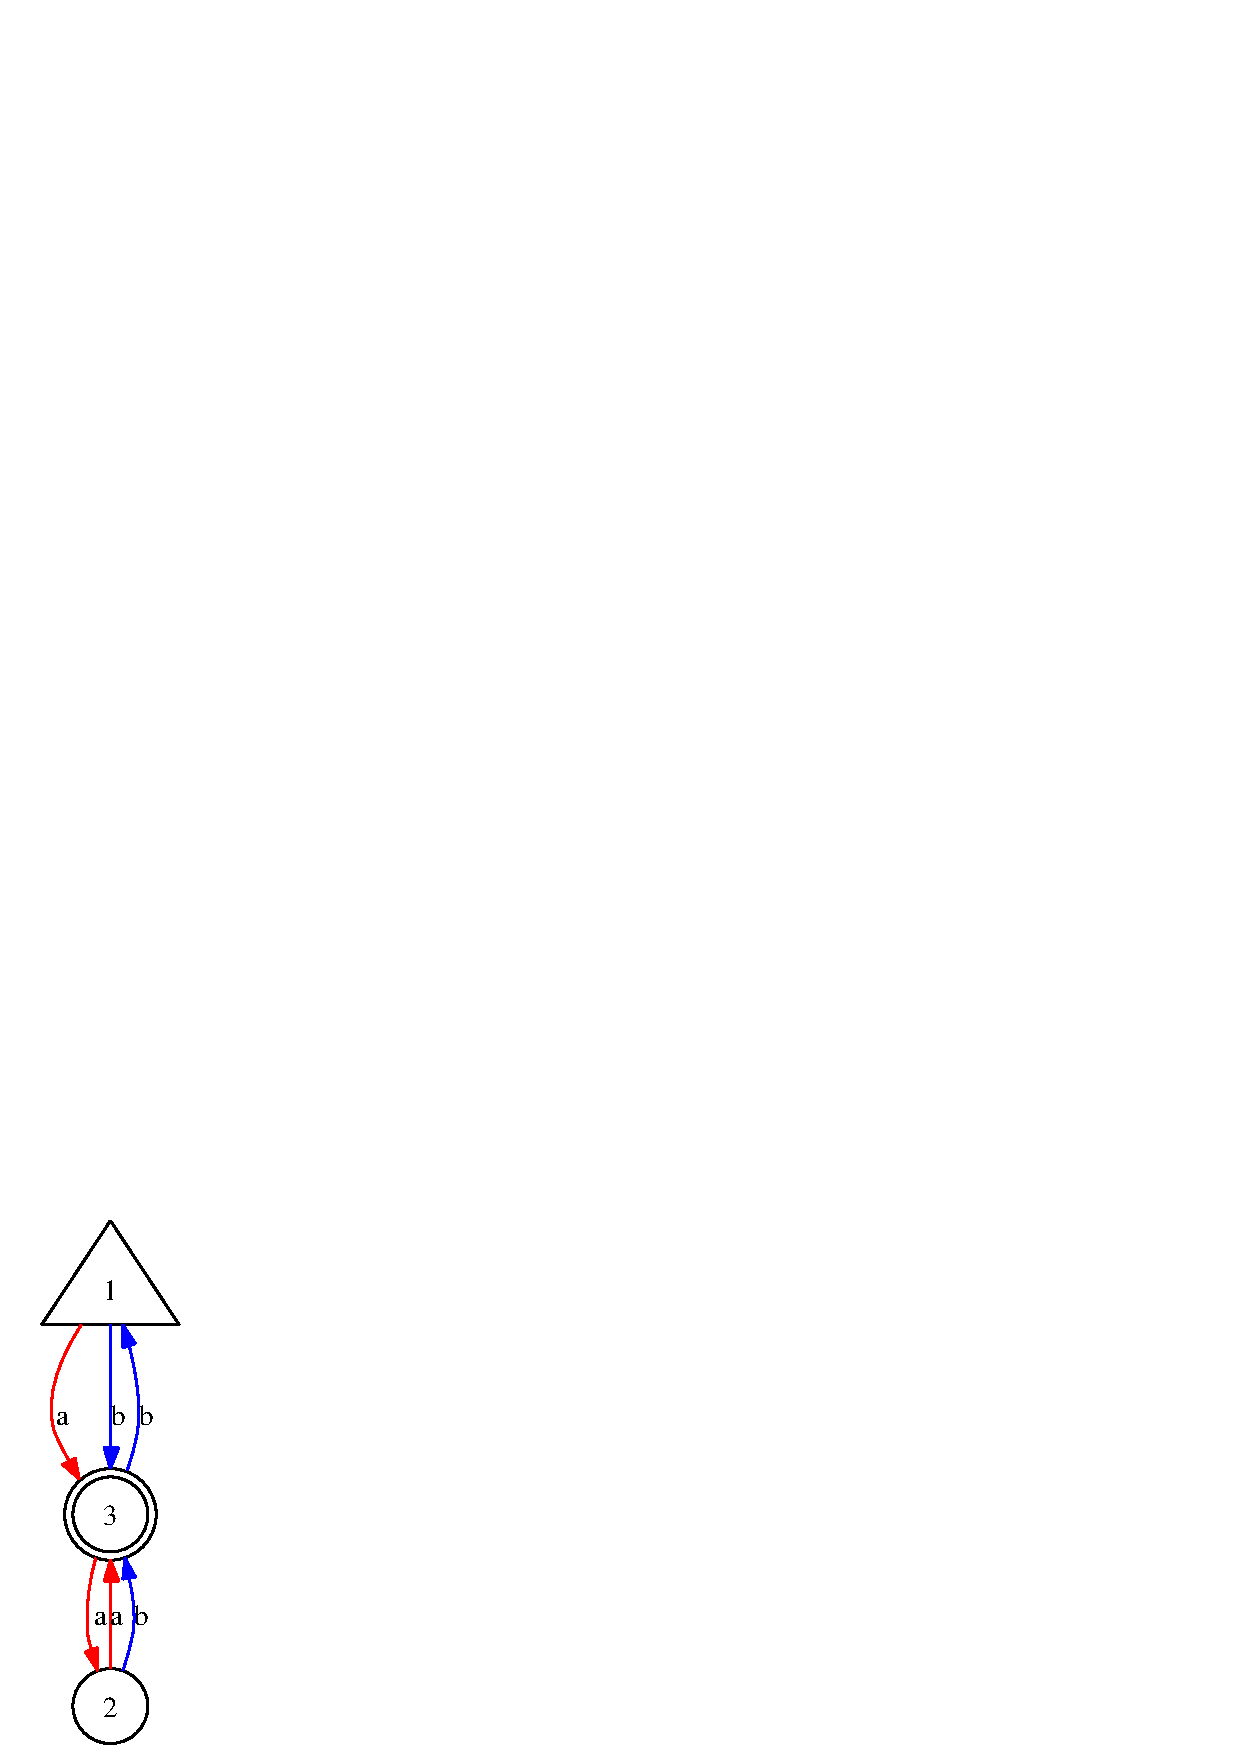
\includegraphics[bb=0 0 132
279]{aut1} \end{center} \label{fig:aut1} \end{figure}   

 This diagram describes a (deterministic) automaton with $ 3 $ states (the elements of the set $ \{1,2,3\}). $ The arrow pointing to the state $ 1 $ indicates that $ 1 $ is the initial state and the two circles around state $ 3 $ indicate that $ 3 $ is a final or accepting state. The set $ \{a,b\} $ is the \emph{alphabet} of the automaton; its elements are called \emph{letters} and are the labels of the edges of the diagram. The words $ a $ , $ ab^2 $ , $ b^5a^3b $ are examples of words recognized by the automaton since they are labels of
paths from the initial to the final state. 

 The set of words recognized by an automaton is called the \emph{language} of the automaton. It is a rational language and may be represented through a
rational expression. For instance, 
\begin{Verbatim}[commandchars=!@|,fontsize=\small,frame=single,label=Example]
  (aUb)(a(aUb)Ub(aUb))*
\end{Verbatim}
 is a rational expression representing the language of the above automaton. 

 Kleene's Theorem states that a language is rational if and only if it is the
language of a finite automaton. Both directions of Kleene's Theorem can be
proved constructively, and these algorithms, to go from an automaton to a
rational expression and \emph{vice-versa}, are implemented in this package. 

 Of course, one has to pay attention to the size of the output produced. When
producing a deterministic automaton equivalent to a given rational expression
one can obtain an optimal solution (the minimal automaton) using standard
algorithms \cite{AHU:74}. 

 When producing a rational expression for the language of an automaton, and
taking into account some reasonable measure for the size of a rational
expression, to determine a minimal one is apparently computationally
difficult. We use here some heuristic methods (to be published elsewhere)
which in practice lead to very reasonable results. 

 The development of this work has benefited from the existence of AMoRE \cite{AMORE:95}, a package written in \texttt{C} to handle Automata, Monoids and Regular Expressions. In fact, its manual has
been very useful and some of the algorithms implemented here are those
implemented in AMoRE. In this package, unlike what happened with AMoRE, we do
not have to worry about the monoid part in order to make it useful to
semigroup theorists, since monoids are already implemented in \textsf{GAP} and we may take advantage of this fact. We just need a function to compute the
transition semigroup of an automaton. 

 

 The parts of this package that have not so directly to do with automata or
rational expressions are put into appendices in this manual. Some words about
these appendices follow. 

 Using the external program Graphviz \cite{KoutsofiosNorth:2002} to graph visualization, one can visualize automata. This very convenient tool
presently works easily under LINUX. 

 Given a finitely generated subgroup of the free group it is possible to
compute a flower automaton and perform Stallings foldings over it in order to
obtain an inverse automaton corresponding to the given subgroup. 

 }

   
\chapter{\textcolor{Chapter }{Finite Automata}}\logpage{[ 2, 0, 0 ]}
\hyperdef{L}{X811E5FC2849C5644}{}
{
 This chapter describes the representations used in this package for finite
automata and some functions to determine information about them. 

 We have to remark that the states of an automaton are always named $1,2,3,\ldots;$ the alphabet may be given by the user. By default it is $\{a,b,c,\ldots\}$ (or $\{a_1,a_2,a_3,\ldots\}$ in the case of alphabets with more than $26$ letters). 

 The transition function of an automaton with $q$ states over an alphabet with $ n$ letters is represented by a (not necessarily dense) $n\times q$ matrix. Each row of the matrix describes the action of the corresponding
letter on the states. In the case of a \emph{deterministic automaton} (DFA) the entries of the matrix are non-negative integers. When all entries of
the transition table are positive integers, the automaton is said to be \emph{dense} or \emph{complete}.  In the case of a \emph{non deterministic automaton} (NFA) the entries of the matrix may be lists of non-negative integers. \emph{Automata with $\epsilon$-transitions} are also allowed: the last letter of the alphabet is assumed to be $\epsilon$ and is represented by @. 
\section{\textcolor{Chapter }{Automata generation}}\logpage{[ 2, 1, 0 ]}
\hyperdef{L}{X821C3B3687B1F2FF}{}
{
  The way to create an automaton in \textsf{GAP} is the following 

\subsection{\textcolor{Chapter }{Automaton}}
\logpage{[ 2, 1, 1 ]}\nobreak
\hyperdef{L}{X87D8222D7B50731E}{}
{\noindent\textcolor{FuncColor}{$\triangleright$\ \ \texttt{Automaton({\mdseries\slshape Type, Size, Alphabet, TransitionTable, Initial, Accepting})\index{Automaton@\texttt{Automaton}}
\label{Automaton}
}\hfill{\scriptsize (function)}}\\


  \texttt{Type} may be \texttt{"det"}, \texttt{"nondet"} or \texttt{"epsilon"} according to whether the automaton is deterministic, non deterministic or an
automaton with $\epsilon$-transitions. \texttt{Size} is a positive integer representing the number of states of the automaton. \texttt{Alphabet} is the number of letters of the alphabet or a list with the letters of the
ordered alphabet. \texttt{TransitionTable} is the transition matrix. The entries are non-negative integers not greater
than the size of the automaton. In the case of non deterministic automata,
lists of non-negative integers not greater than the size of the automaton are
also allowed. \texttt{Initial} and \texttt{Accepting} are, respectively, the lists of initial and accepting states. 
\begin{Verbatim}[commandchars=!@B,fontsize=\small,frame=single,label=Example]
  
  !gapprompt@gap>B !gapinput@aut:=Automaton("det",4,2,[[3,,3,4],[3,4,0,4]],[1],[4]);B
  < deterministic automaton on 2 letters with 4 states >
  !gapprompt@gap>B !gapinput@Display(aut);B
     |  1  2  3  4
  -----------------
   a |  3     3  4
   b |  3  4     4
  Initial state:   [ 1 ]
  Accepting state: [ 4 ]
  
\end{Verbatim}
 The alphabet of the automaton may be specified: 
\begin{Verbatim}[commandchars=!@B,fontsize=\small,frame=single,label=Example]
  !gapprompt@gap>B !gapinput@aut:=Automaton("det",4,"01",[[3,,3,4],[3,4,0,4]],[1],[4]);B
  < deterministic automaton on 2 letters with 4 states >
  !gapprompt@gap>B !gapinput@Display(aut);B
     |  1  2  3  4
  -----------------
   0 |  3     3  4
   1 |  3  4     4
  Initial state:   [ 1 ]
  Accepting state: [ 4 ]
\end{Verbatim}
 Instead of leaving a hole in the transition matrix, we may write a \texttt{0} to mean that no transition is present. Non deterministic automata may be given
the same way. 
\begin{Verbatim}[commandchars=!@B,fontsize=\small,frame=single,label=Example]
  !gapprompt@gap>B !gapinput@ndaut:=Automaton("nondet",4,2,[[3,[1,2],3,0],[3,4,0,[2,3]]],[1],[4]);B
  < non deterministic automaton on 2 letters with 4 states >
  !gapprompt@gap>B !gapinput@Display(ndaut);B
     |  1       2          3       4
  -----------------------------------------
   a | [ 3 ]   [ 1, 2 ]   [ 3 ]
   b | [ 3 ]   [ 4 ]              [ 2, 3 ]
  Initial state:   [ 1 ]
  Accepting state: [ 4 ]
\end{Verbatim}
 Also in the same way can be given $\epsilon$-automata. The letter $\epsilon$ is written \texttt{@} instead. 
\begin{Verbatim}[commandchars=!BC,fontsize=\small,frame=single,label=Example]
  !gappromptBgap>C !gapinputBx:=Automaton("epsilon",3,"01@",[[,[2],[3]],[[1,3],,[1]],[[1],[2],C
  !gappromptB>C !gapinputB[2]]],[2],[2,3]);C
  < epsilon automaton on 3 letters with 3 states >
  !gappromptBgap>C !gapinputBDisplay(x);C
     |  1          2       3
  ------------------------------
   0 |            [ 2 ]   [ 3 ]
   1 | [ 1, 3 ]           [ 1 ]
   @ | [ 1 ]      [ 2 ]   [ 2 ]
  Initial state:    [ 2 ]
  Accepting states: [ 2, 3 ]
\end{Verbatim}
 Bigger automata are displayed in another form: 
\begin{Verbatim}[commandchars=!@|,fontsize=\small,frame=single,label=Example]
  !gapprompt@gap>| !gapinput@aut:=Automaton("det",16,2,[[4,0,0,6,3,1,4,8,7,4,3,0,6,1,6,0],|
  !gapprompt@>| !gapinput@[3,4,0,0,6,1,0,6,1,6,1,6,6,4,8,7,4,5]],[1],[4]);|
  < deterministic automaton on 2 letters with 16 states >
  !gapprompt@gap>| !gapinput@Display(aut);|
  1    a   4
  1    b   3
  2    b   4
      ... some more lines
  15   a   6
  15   b   8
  16   b   7
  Initial state:   [ 1 ]
  Accepting state: [ 4 ]
\end{Verbatim}
 }

 

\subsection{\textcolor{Chapter }{IsAutomaton}}
\logpage{[ 2, 1, 2 ]}\nobreak
\hyperdef{L}{X83CCDEF9814F1E6D}{}
{\noindent\textcolor{FuncColor}{$\triangleright$\ \ \texttt{IsAutomaton({\mdseries\slshape O})\index{IsAutomaton@\texttt{IsAutomaton}}
\label{IsAutomaton}
}\hfill{\scriptsize (function)}}\\


 In the presence of an object \mbox{\texttt{\mdseries\slshape O}}, one may want to test whether \texttt{O} is an automaton. This may be done using the function \texttt{IsAutomaton}. 
\begin{Verbatim}[commandchars=!@|,fontsize=\small,frame=single,label=Example]
  !gapprompt@gap>| !gapinput@x:=Automaton("det",3,2,[ [ 0, 2, 0 ], [ 0, 1, 0 ] ],[ 3 ],[ 2 ]);;|
  !gapprompt@gap>| !gapinput@IsAutomaton(x);|
  true
\end{Verbatim}
 }

 

\subsection{\textcolor{Chapter }{IsDeterministicAutomaton}}
\logpage{[ 2, 1, 3 ]}\nobreak
\hyperdef{L}{X7D39CECC7E12DD8A}{}
{\noindent\textcolor{FuncColor}{$\triangleright$\ \ \texttt{IsDeterministicAutomaton({\mdseries\slshape aut})\index{IsDeterministicAutomaton@\texttt{IsDeterministicAutomaton}}
\label{IsDeterministicAutomaton}
}\hfill{\scriptsize (function)}}\\


 Returns \texttt{true} when \texttt{aut} is a deterministic automaton and \texttt{false} otherwise. 
\begin{Verbatim}[commandchars=!@|,fontsize=\small,frame=single,label=Example]
  !gapprompt@gap>| !gapinput@x:=Automaton("det",3,2,[ [ 0, 2, 0 ], [ 0, 1, 0 ] ],[ 3 ],[ 2 ]);;|
  !gapprompt@gap>| !gapinput@IsDeterministicAutomaton(x);|
  true
\end{Verbatim}
 }

  

\subsection{\textcolor{Chapter }{IsNonDeterministicAutomaton}}
\logpage{[ 2, 1, 4 ]}\nobreak
\hyperdef{L}{X83C1148481BAA3DD}{}
{\noindent\textcolor{FuncColor}{$\triangleright$\ \ \texttt{IsNonDeterministicAutomaton({\mdseries\slshape aut})\index{IsNonDeterministicAutomaton@\texttt{IsNonDeterministicAutomaton}}
\label{IsNonDeterministicAutomaton}
}\hfill{\scriptsize (function)}}\\


 Returns \texttt{true} when \texttt{aut} is a non deterministic automaton and \texttt{false} otherwise. 
\begin{Verbatim}[commandchars=!@|,fontsize=\small,frame=single,label=Example]
  !gapprompt@gap>| !gapinput@y:=Automaton("nondet",3,2,[[,[1,3],],[,[2,3],[1,3]]],[1,2],[1,3]);;|
  !gapprompt@gap>| !gapinput@IsNonDeterministicAutomaton(y);|
  true
\end{Verbatim}
 }

 

\subsection{\textcolor{Chapter }{IsEpsilonAutomaton}}
\logpage{[ 2, 1, 5 ]}\nobreak
\hyperdef{L}{X81EC5331790D6022}{}
{\noindent\textcolor{FuncColor}{$\triangleright$\ \ \texttt{IsEpsilonAutomaton({\mdseries\slshape aut})\index{IsEpsilonAutomaton@\texttt{IsEpsilonAutomaton}}
\label{IsEpsilonAutomaton}
}\hfill{\scriptsize (function)}}\\


 Returns \texttt{true} when \texttt{aut} is an $\epsilon$-automaton and \texttt{false} otherwise. 
\begin{Verbatim}[commandchars=!@|,fontsize=\small,frame=single,label=Example]
  !gapprompt@gap>| !gapinput@z:=Automaton("epsilon",2,2,[[[1,2],],[[2],[1]]],[1,2],[1,2]);;|
  !gapprompt@gap>| !gapinput@IsEpsilonAutomaton(z);|
  true
\end{Verbatim}
 }

 

\subsection{\textcolor{Chapter }{String}}
\logpage{[ 2, 1, 6 ]}\nobreak
\hyperdef{L}{X81FB5BE27903EC32}{}
{\noindent\textcolor{FuncColor}{$\triangleright$\ \ \texttt{String({\mdseries\slshape aut})\index{String@\texttt{String}}
\label{String}
}\hfill{\scriptsize (function)}}\\


 The way \textsf{GAP} displays an automaton is quite natural, but when one wants to do small
changes, for example using \emph{copy/paste}, the use of the function \texttt{String} (possibly followed by \texttt{Print}) may be usefull. 
\begin{Verbatim}[commandchars=!@|,fontsize=\small,frame=single,label=Example]
  !gapprompt@gap>| !gapinput@x:=Automaton("det",3,2,[ [ 0, 2, 0 ], [ 0, 1, 0 ] ],[ 3 ],[ 2 ]);;|
  !gapprompt@gap>| !gapinput@String(x);|
  "Automaton(\"det\",3,\"ab\",[ [ 0, 2, 0 ], [ 0, 1, 0 ] ],[ 3 ],[ 2 ]);;"
  !gapprompt@gap>| !gapinput@Print(String(x));|
  Automaton("det",3,"ab",[ [ 0, 2, 0 ], [ 0, 1, 0 ] ],[ 3 ],[ 2 ]);;
\end{Verbatim}
 
\begin{Verbatim}[commandchars=!|B,fontsize=\small,frame=single,label=Example]
  !gapprompt|gap>B !gapinput|z:=Automaton("epsilon",2,2,[[[1,2],],[[2],[1]]],[1,2],[1,2]);;B
  !gapprompt|gap>B !gapinput|Print(String(z));B
  Automaton("epsilon",2,"a@",[ [ [ 1, 2 ], [ ] ], [ [ 2 ], [ 1 ] ] ],[ 1, 2 ],[ \
  1, 2 ]);;
\end{Verbatim}
 }

 

\subsection{\textcolor{Chapter }{RandomAutomaton}}
\logpage{[ 2, 1, 7 ]}\nobreak
\hyperdef{L}{X801019097C93BCCC}{}
{\noindent\textcolor{FuncColor}{$\triangleright$\ \ \texttt{RandomAutomaton({\mdseries\slshape Type, Size, Alphabet})\index{RandomAutomaton@\texttt{RandomAutomaton}}
\label{RandomAutomaton}
}\hfill{\scriptsize (function)}}\\


 Given the \mbox{\texttt{\mdseries\slshape Type}}, the \mbox{\texttt{\mdseries\slshape Size}} (i.e. the number of states) and the \mbox{\texttt{\mdseries\slshape Alphabet}} (a positive integer or a list), returns a pseudo random automaton with these
parameters. 
\begin{Verbatim}[commandchars=!BC,fontsize=\small,frame=single,label=Example]
  !gappromptBgap>C !gapinputBRandomAutomaton("det",5,"ac");C
  < deterministic automaton on 2 letters with 5 states >
  !gappromptBgap>C !gapinputBDisplay(last);C
     |  1  2  3  4  5
  --------------------
   a |     2  3
   c |  2  3
  Initial state:    [ 4 ]
  Accepting states: [ 3, 4 ]
  
  !gappromptBgap>C !gapinputBRandomAutomaton("nondet",3,["a","b","c"]);C
  < non deterministic automaton on 3 letters with 3 states >
  
  !gappromptBgap>C !gapinputBRandomAutomaton("epsilon",2,"abc");C
  < epsilon automaton on 4 letters with 2 states >
  
  !gappromptBgap>C !gapinputBRandomAutomaton("epsilon",2,2);C
  < epsilon automaton on 3 letters with 2 states >
  !gappromptBgap>C !gapinputBDisplay(last);C
     |  1          2
  ----------------------
   a | [ 1, 2 ]
   b | [ 2 ]      [ 1 ]
   @ | [ 1, 2 ]
  Initial state:    [ 2 ]
  Accepting states: [ 1, 2 ]
  
  !gappromptBgap>C !gapinputBa:=RandomTransformation(3);;C
  !gappromptBgap>C !gapinputBb:=RandomTransformation(3);;C
  !gappromptBgap>C !gapinputBaut:=RandomAutomaton("det",4,[a,b]);C
  < deterministic automaton on 2 letters with 4 states >
\end{Verbatim}
 }

 }

 
\section{\textcolor{Chapter }{Automata internals}}\logpage{[ 2, 2, 0 ]}
\hyperdef{L}{X80AB906D86BBC153}{}
{
 In this section we describe the functions used to access the internals of an
automaton. 

\subsection{\textcolor{Chapter }{AlphabetOfAutomaton}}
\logpage{[ 2, 2, 1 ]}\nobreak
\hyperdef{L}{X7A34B47778B50FFE}{}
{\noindent\textcolor{FuncColor}{$\triangleright$\ \ \texttt{AlphabetOfAutomaton({\mdseries\slshape aut})\index{AlphabetOfAutomaton@\texttt{AlphabetOfAutomaton}}
\label{AlphabetOfAutomaton}
}\hfill{\scriptsize (function)}}\\


 Returns the number of symbols in the alphabet of automaton \texttt{aut}. 
\begin{Verbatim}[commandchars=!@|,fontsize=\small,frame=single,label=Example]
  !gapprompt@gap>| !gapinput@aut:=Automaton("det",4,2,[[3,,3,4],[3,4,0,]],[1],[4]);;|
  !gapprompt@gap>| !gapinput@AlphabetOfAutomaton(aut);|
  2
\end{Verbatim}
 }

 

\subsection{\textcolor{Chapter }{AlphabetOfAutomatonAsList}}
\logpage{[ 2, 2, 2 ]}\nobreak
\hyperdef{L}{X8044B24B82C59BBF}{}
{\noindent\textcolor{FuncColor}{$\triangleright$\ \ \texttt{AlphabetOfAutomatonAsList({\mdseries\slshape aut})\index{AlphabetOfAutomatonAsList@\texttt{AlphabetOfAutomatonAsList}}
\label{AlphabetOfAutomatonAsList}
}\hfill{\scriptsize (function)}}\\


 Returns the alphabet of automaton \texttt{aut} always as a list. Note that when the alphabet of the automaton is given as an
integer (meaning the number of symbols) not greater than 26 it returns the
list \texttt{"abcd...."}. If the alphabet is given by means of an integer greater than 26, the
function returns \texttt{[ "a1", "a2", "a3", "a4", ... ]}. 
\begin{Verbatim}[commandchars=!@|,fontsize=\small,frame=single,label=Example]
  !gapprompt@gap>| !gapinput@a:=RandomAutomaton("det",5,"cat");|
  < deterministic automaton on 3 letters with 5 states >
  !gapprompt@gap>| !gapinput@AlphabetOfAutomaton(a);|
  3
  !gapprompt@gap>| !gapinput@AlphabetOfAutomatonAsList(a);|
  "cat"
  !gapprompt@gap>| !gapinput@a:=RandomAutomaton("det",5,20);|
  < deterministic automaton on 20 letters with 5 states >
  !gapprompt@gap>| !gapinput@AlphabetOfAutomaton(a);|
  20
  !gapprompt@gap>| !gapinput@AlphabetOfAutomatonAsList(a);|
  "abcdefghijklmnopqrst"
  !gapprompt@gap>| !gapinput@a:=RandomAutomaton("det",5,30);|
  < deterministic automaton on 30 letters with 5 states >
  !gapprompt@gap>| !gapinput@AlphabetOfAutomaton(a);|
  30
  !gapprompt@gap>| !gapinput@AlphabetOfAutomatonAsList(a);|
  [ "a1", "a2", "a3", "a4", "a5", "a6", "a7", "a8", "a9", "a10", "a11", 
    "a12", "a13", "a14", "a15", "a16", "a17", "a18", "a19", "a20", "a21",
    "a22", "a23", "a24", "a25", "a26", "a27", "a28", "a29", "a30" ]
\end{Verbatim}
 }

 

\subsection{\textcolor{Chapter }{TransitionMatrixOfAutomaton}}
\logpage{[ 2, 2, 3 ]}\nobreak
\hyperdef{L}{X872BB42A81E4D0E7}{}
{\noindent\textcolor{FuncColor}{$\triangleright$\ \ \texttt{TransitionMatrixOfAutomaton({\mdseries\slshape aut})\index{TransitionMatrixOfAutomaton@\texttt{TransitionMatrixOfAutomaton}}
\label{TransitionMatrixOfAutomaton}
}\hfill{\scriptsize (function)}}\\


 Returns the transition matrix of automaton \texttt{aut}. 
\begin{Verbatim}[commandchars=!@|,fontsize=\small,frame=single,label=Example]
  !gapprompt@gap>| !gapinput@aut:=Automaton("det",4,2,[[3,,3,4],[3,4,0,]],[1],[4]);;|
  !gapprompt@gap>| !gapinput@TransitionMatrixOfAutomaton(aut);|
  [ [ 3, 0, 3, 4 ], [ 3, 4, 0, 0 ] ]
\end{Verbatim}
 }

 

\subsection{\textcolor{Chapter }{InitialStatesOfAutomaton}}
\logpage{[ 2, 2, 4 ]}\nobreak
\hyperdef{L}{X7B5C3CFA83FF80EA}{}
{\noindent\textcolor{FuncColor}{$\triangleright$\ \ \texttt{InitialStatesOfAutomaton({\mdseries\slshape aut})\index{InitialStatesOfAutomaton@\texttt{InitialStatesOfAutomaton}}
\label{InitialStatesOfAutomaton}
}\hfill{\scriptsize (function)}}\\


 Returns the initial states of automaton \texttt{aut}. 
\begin{Verbatim}[commandchars=!@|,fontsize=\small,frame=single,label=Example]
  !gapprompt@gap>| !gapinput@aut:=Automaton("det",4,2,[[3,,3,4],[3,4,0,]],[1],[4]);;|
  !gapprompt@gap>| !gapinput@InitialStatesOfAutomaton(aut);|
  [ 1 ]
\end{Verbatim}
 }

 

\subsection{\textcolor{Chapter }{SetInitialStatesOfAutomaton}}
\logpage{[ 2, 2, 5 ]}\nobreak
\hyperdef{L}{X8408FE8487028B7F}{}
{\noindent\textcolor{FuncColor}{$\triangleright$\ \ \texttt{SetInitialStatesOfAutomaton({\mdseries\slshape aut, I})\index{SetInitialStatesOfAutomaton@\texttt{SetInitialStatesOfAutomaton}}
\label{SetInitialStatesOfAutomaton}
}\hfill{\scriptsize (function)}}\\


 Sets the initial states of automaton \texttt{aut}. \texttt{I} may be a positive integer or a list of positive integers. 
\begin{Verbatim}[commandchars=!@|,fontsize=\small,frame=single,label=Example]
  !gapprompt@gap>| !gapinput@aut:=Automaton("det",4,2,[[3,,3,4],[3,4,0,]],[1],[4]);;|
  !gapprompt@gap>| !gapinput@SetInitialStatesOfAutomaton(aut,4);|
  !gapprompt@gap>| !gapinput@InitialStatesOfAutomaton(aut);|
  [ 4 ]
  !gapprompt@gap>| !gapinput@SetInitialStatesOfAutomaton(aut,[2,3]);|
  !gapprompt@gap>| !gapinput@InitialStatesOfAutomaton(aut);|
  [ 2, 3 ]
\end{Verbatim}
 }

 

\subsection{\textcolor{Chapter }{FinalStatesOfAutomaton}}
\logpage{[ 2, 2, 6 ]}\nobreak
\hyperdef{L}{X78CDDCC27D085F00}{}
{\noindent\textcolor{FuncColor}{$\triangleright$\ \ \texttt{FinalStatesOfAutomaton({\mdseries\slshape aut})\index{FinalStatesOfAutomaton@\texttt{FinalStatesOfAutomaton}}
\label{FinalStatesOfAutomaton}
}\hfill{\scriptsize (function)}}\\


 Returns the final states of automaton \texttt{aut}. 
\begin{Verbatim}[commandchars=!@|,fontsize=\small,frame=single,label=Example]
  !gapprompt@gap>| !gapinput@aut:=Automaton("det",4,2,[[3,,3,4],[3,4,0,]],[1],[4]);;|
  !gapprompt@gap>| !gapinput@FinalStatesOfAutomaton(aut);|
  [ 4 ]
\end{Verbatim}
 }

 

\subsection{\textcolor{Chapter }{SetFinalStatesOfAutomaton}}
\logpage{[ 2, 2, 7 ]}\nobreak
\hyperdef{L}{X80689F1480F9D959}{}
{\noindent\textcolor{FuncColor}{$\triangleright$\ \ \texttt{SetFinalStatesOfAutomaton({\mdseries\slshape aut, F})\index{SetFinalStatesOfAutomaton@\texttt{SetFinalStatesOfAutomaton}}
\label{SetFinalStatesOfAutomaton}
}\hfill{\scriptsize (function)}}\\


 Sets the final states of automaton \texttt{aut}. \texttt{F} may be a positive integer or a list of positive integers. 
\begin{Verbatim}[commandchars=!@|,fontsize=\small,frame=single,label=Example]
  !gapprompt@gap>| !gapinput@aut:=Automaton("det",4,2,[[3,,3,4],[3,4,0,]],[1],[4]);;|
  !gapprompt@gap>| !gapinput@FinalStatesOfAutomaton(aut);|
  [ 4 ]
  !gapprompt@gap>| !gapinput@SetFinalStatesOfAutomaton(aut,2);|
  !gapprompt@gap>| !gapinput@FinalStatesOfAutomaton(aut);|
  [ 2 ]
\end{Verbatim}
 }

 

\subsection{\textcolor{Chapter }{NumberStatesOfAutomaton}}
\logpage{[ 2, 2, 8 ]}\nobreak
\hyperdef{L}{X7D22AD207A3D5FF4}{}
{\noindent\textcolor{FuncColor}{$\triangleright$\ \ \texttt{NumberStatesOfAutomaton({\mdseries\slshape aut})\index{NumberStatesOfAutomaton@\texttt{NumberStatesOfAutomaton}}
\label{NumberStatesOfAutomaton}
}\hfill{\scriptsize (function)}}\\


 Returns the number of states of automaton \texttt{aut}. 
\begin{Verbatim}[commandchars=!@|,fontsize=\small,frame=single,label=Example]
  !gapprompt@gap>| !gapinput@aut:=Automaton("det",4,2,[[3,,3,4],[3,4,0,]],[1],[4]);;|
  !gapprompt@gap>| !gapinput@NumberStatesOfAutomaton(aut);|
  4
\end{Verbatim}
 }

 }

 
\section{\textcolor{Chapter }{Comparison of automata}}\logpage{[ 2, 3, 0 ]}
\hyperdef{L}{X8454E24E7D9FC1C2}{}
{
 Although there is no standard way to compare automata it is usefull to be able
to do some kind of comparison. Doing so, one can consider sets of automata. We
just compare the strings of the automata. 
\begin{Verbatim}[commandchars=!@|,fontsize=\small,frame=single,label=Example]
  !gapprompt@gap>| !gapinput@x:=Automaton("det",3,2,[ [ 0, 2, 0 ], [ 0, 1, 0 ] ],[ 3 ],[ 2 ]);;|
  !gapprompt@gap>| !gapinput@y:=Automaton("det",3,2,[ [ 2, 0, 0 ], [ 1, 3, 0 ] ],[ 3 ],[ 2, 3 ]);;|
  !gapprompt@gap>| !gapinput@x=y;|
  false
  !gapprompt@gap>| !gapinput@Size(Set([y,x,x]));|
  2
\end{Verbatim}
 }

 
\section{\textcolor{Chapter }{Tests involving automata}}\logpage{[ 2, 4, 0 ]}
\hyperdef{L}{X867887A683961C63}{}
{
 This section describes some useful tests involving automata. 

\subsection{\textcolor{Chapter }{IsDenseAutomaton}}
\logpage{[ 2, 4, 1 ]}\nobreak
\hyperdef{L}{X8356E41086482483}{}
{\noindent\textcolor{FuncColor}{$\triangleright$\ \ \texttt{IsDenseAutomaton({\mdseries\slshape aut})\index{IsDenseAutomaton@\texttt{IsDenseAutomaton}}
\label{IsDenseAutomaton}
}\hfill{\scriptsize (function)}}\\


 Tests whether a deterministic automaton \texttt{aut} is complete. (See also \texttt{NullCompletionAutomaton} (\ref{NullCompletionAutomaton}).) 
\begin{Verbatim}[commandchars=!@|,fontsize=\small,frame=single,label=Example]
  !gapprompt@gap>| !gapinput@aut:=Automaton("det",4,2,[[3,,3,4],[3,4,0,]],[1],[4]);;|
  !gapprompt@gap>| !gapinput@IsDenseAutomaton(aut);                                 |
  false
\end{Verbatim}
 }

 

\subsection{\textcolor{Chapter }{IsRecognizedByAutomaton}}
\logpage{[ 2, 4, 2 ]}\nobreak
\hyperdef{L}{X8676D8388053F1E7}{}
{\noindent\textcolor{FuncColor}{$\triangleright$\ \ \texttt{IsRecognizedByAutomaton({\mdseries\slshape A, w})\index{IsRecognizedByAutomaton@\texttt{IsRecognizedByAutomaton}}
\label{IsRecognizedByAutomaton}
}\hfill{\scriptsize (function)}}\\


 The arguments are: an automaton \mbox{\texttt{\mdseries\slshape A}} and a string (i.e. a word) \mbox{\texttt{\mdseries\slshape w}} in the alphabet of the automaton. Returns \texttt{true} if the word is recognized by the automaton and \texttt{false} otherwise. 
\begin{Verbatim}[commandchars=!@|,fontsize=\small,frame=single,label=Example]
  !gapprompt@gap>| !gapinput@aut:=Automaton("det",3,2,[[1,2,1],[2,1,3]],[1],[2]);;|
  !gapprompt@gap>| !gapinput@IsRecognizedByAutomaton(aut,"bbb");|
  true
  
  !gapprompt@gap>| !gapinput@aut:=Automaton("det",3,"01",[[1,2,1],[2,1,3]],[1],[2]);;|
  !gapprompt@gap>| !gapinput@IsRecognizedByAutomaton(aut,"111");|
  true
\end{Verbatim}
 }

 

\subsection{\textcolor{Chapter }{IsPermutationAutomaton}}
\logpage{[ 2, 4, 3 ]}\nobreak
\hyperdef{L}{X80CCDD438258CD25}{}
{\noindent\textcolor{FuncColor}{$\triangleright$\ \ \texttt{IsPermutationAutomaton({\mdseries\slshape aut})\index{IsPermutationAutomaton@\texttt{IsPermutationAutomaton}}
\label{IsPermutationAutomaton}
}\hfill{\scriptsize (function)}}\\


 The argument is a deterministic automaton. Returns \texttt{true} when each letter of the alphabet induces a permutation on the vertices and \texttt{false} otherwise. 
\begin{Verbatim}[commandchars=!@|,fontsize=\small,frame=single,label=Example]
  !gapprompt@gap>| !gapinput@x:=Automaton("det",3,2,[ [ 1, 2, 3 ], [ 1, 2, 3 ] ],[ 1 ],[ 2, 3 ]);;|
  !gapprompt@gap>| !gapinput@IsPermutationAutomaton(x);|
  true
\end{Verbatim}
 }

 

\subsection{\textcolor{Chapter }{IsInverseAutomaton}}
\logpage{[ 2, 4, 4 ]}\nobreak
\hyperdef{L}{X7B7CA23680888C9C}{}
{\noindent\textcolor{FuncColor}{$\triangleright$\ \ \texttt{IsInverseAutomaton({\mdseries\slshape aut})\index{IsInverseAutomaton@\texttt{IsInverseAutomaton}}
\label{IsInverseAutomaton}
}\hfill{\scriptsize (function)}}\\


 The argument is a deterministic automaton. Returns \texttt{true} when each letter of the alphabet induces an injective partial function on the
vertices and \texttt{false} otherwise. 
\begin{Verbatim}[commandchars=!@|,fontsize=\small,frame=single,label=Example]
  !gapprompt@gap>| !gapinput@x:=Automaton("det",3,2,[ [ 0, 1, 3 ], [ 0, 1, 2 ] ],[ 2 ],[ 1 ]);;|
  !gapprompt@gap>| !gapinput@IsInverseAutomaton(x);|
  true
\end{Verbatim}
 Frequently an inverse automaton is thought as if the inverse edges (labeled by
formal inverses of the letters of the alphabet) were present, although they
are usually not explicited. They can be made explicit using the function \texttt{AddInverseEdgesToInverseAutomaton} }

 

\subsection{\textcolor{Chapter }{AddInverseEdgesToInverseAutomaton}}
\logpage{[ 2, 4, 5 ]}\nobreak
\hyperdef{L}{X7A4CDEFB84B97849}{}
{\noindent\textcolor{FuncColor}{$\triangleright$\ \ \texttt{AddInverseEdgesToInverseAutomaton({\mdseries\slshape aut})\index{AddInverseEdgesToInverseAutomaton@\texttt{AddInverseEdgesToInverseAutomaton}}
\label{AddInverseEdgesToInverseAutomaton}
}\hfill{\scriptsize (function)}}\\


 The argument is an inverse automaton over the alphabet $\{a,b,c,\ldots\}$. Returns an automaton with the inverse edges added. (The formal inverse of a
letter is represented by the corresponding capital letter.) 
\begin{Verbatim}[commandchars=!@C,fontsize=\small,frame=single,label=Example]
  !gapprompt@gap>C !gapinput@x:=Automaton("det",3,2,[[ 0, 1, 3 ],[ 0, 1, 2 ]],[ 2 ],[ 1 ]);;Display(x);C
     |  1  2  3
  --------------
   a |     1  3
   b |     1  2
  Initial state:   [ 2 ]
  Accepting state: [ 1 ]
  !gapprompt@gap>C !gapinput@AddInverseEdgesToInverseAutomaton(x);Display(x);C
     |  1  2  3
  --------------
   a |     1  3
   b |     1  2
   A |  2     3
   B |  2  3
  Initial state:   [ 2 ]
  Accepting state: [ 1 ]
\end{Verbatim}
 }

 

\subsection{\textcolor{Chapter }{IsReversibleAutomaton}}
\logpage{[ 2, 4, 6 ]}\nobreak
\hyperdef{L}{X8321BCE57E55FB30}{}
{\noindent\textcolor{FuncColor}{$\triangleright$\ \ \texttt{IsReversibleAutomaton({\mdseries\slshape aut})\index{IsReversibleAutomaton@\texttt{IsReversibleAutomaton}}
\label{IsReversibleAutomaton}
}\hfill{\scriptsize (function)}}\\


 The argument is a deterministic automaton. Returns \texttt{true} when \mbox{\texttt{\mdseries\slshape aut}} is a reversible automaton, i.e. the automaton obtained by reversing all edges
and switching the initial and final states (see also \texttt{ReversedAutomaton} (\ref{ReversedAutomaton})) is deterministic. Returns \texttt{false} otherwise. 
\begin{Verbatim}[commandchars=!@|,fontsize=\small,frame=single,label=Example]
  !gapprompt@gap>| !gapinput@x:=Automaton("det",3,2,[ [ 0, 1, 2 ], [ 0, 1, 3 ] ],[ 2 ],[ 2 ]);;|
  !gapprompt@gap>| !gapinput@IsReversibleAutomaton(x);|
  true
\end{Verbatim}
 }

 }

 
\section{\textcolor{Chapter }{Basic operations}}\logpage{[ 2, 5, 0 ]}
\hyperdef{L}{X82EB5BE77F9F686A}{}
{
 

\subsection{\textcolor{Chapter }{CopyAutomaton}}
\logpage{[ 2, 5, 1 ]}\nobreak
\hyperdef{L}{X8225A1B886131707}{}
{\noindent\textcolor{FuncColor}{$\triangleright$\ \ \texttt{CopyAutomaton({\mdseries\slshape aut})\index{CopyAutomaton@\texttt{CopyAutomaton}}
\label{CopyAutomaton}
}\hfill{\scriptsize (function)}}\\


 Returns a new automaton, which is a copy of automaton \mbox{\texttt{\mdseries\slshape aut}}. }

 

\subsection{\textcolor{Chapter }{NullCompletionAutomaton}}
\logpage{[ 2, 5, 2 ]}\nobreak
\hyperdef{L}{X80D423A584246E2E}{}
{\noindent\textcolor{FuncColor}{$\triangleright$\ \ \texttt{NullCompletionAutomaton({\mdseries\slshape aut})\index{NullCompletionAutomaton@\texttt{NullCompletionAutomaton}}
\label{NullCompletionAutomaton}
}\hfill{\scriptsize (function)}}\\


 \texttt{aut} is a deterministic automaton. If it is complete returns \mbox{\texttt{\mdseries\slshape aut}}, otherwise returns the completion (with a null state) of \mbox{\texttt{\mdseries\slshape aut}}. Notice that the words recognized by \mbox{\texttt{\mdseries\slshape aut}} and its completion are the same. 
\begin{Verbatim}[commandchars=!@B,fontsize=\small,frame=single,label=Example]
  !gapprompt@gap>B !gapinput@aut:=Automaton("det",4,2,[[3,,3,4],[2,4,4,]],[1],[4]);;B
  !gapprompt@gap>B !gapinput@IsDenseAutomaton(aut);B
  false
  !gapprompt@gap>B !gapinput@y:=NullCompletionAutomaton(aut);;Display(y);B
     |  1  2  3  4  5
  --------------------
   a |  3  5  3  4  5
   b |  2  4  4  5  5
  Initial state:   [ 1 ]
  Accepting state: [ 4 ]
\end{Verbatim}
 The state added is a \emph{sink state} i.e. it is a state $q$ which is not initial nor accepting and for all letter $a$ in the alphabet of the automaton, $q$ is the result of the action of $a$ in $q$. (Notice that reading a word, one does not go out of a sink state.) }

 

\subsection{\textcolor{Chapter }{ListSinkStatesAut}}
\logpage{[ 2, 5, 3 ]}\nobreak
\hyperdef{L}{X79F052EC81135807}{}
{\noindent\textcolor{FuncColor}{$\triangleright$\ \ \texttt{ListSinkStatesAut({\mdseries\slshape aut})\index{ListSinkStatesAut@\texttt{ListSinkStatesAut}}
\label{ListSinkStatesAut}
}\hfill{\scriptsize (function)}}\\


 Computes the list of all sink states of the automaton \mbox{\texttt{\mdseries\slshape aut}}. 
\begin{Verbatim}[commandchars=!@|,fontsize=\small,frame=single,label=Example]
  !gapprompt@gap>| !gapinput@x:=Automaton("det",3,2,[ [ 2, 3, 3 ], [ 1, 2, 3 ] ],[ 1 ],[ 2, 3 ]);;|
  !gapprompt@gap>| !gapinput@ListSinkStatesAut(x);|
  [  ]
  !gapprompt@gap>| !gapinput@y:=Automaton("det",3,2,[ [ 2, 3, 3 ], [ 1, 2, 3 ] ],[ 1 ],[ 2 ]);;|
  !gapprompt@gap>| !gapinput@ListSinkStatesAut(y);|
  [ 3 ]
\end{Verbatim}
 }

 

\subsection{\textcolor{Chapter }{RemovedSinkStates}}
\logpage{[ 2, 5, 4 ]}\nobreak
\hyperdef{L}{X8240136E7A26B1A6}{}
{\noindent\textcolor{FuncColor}{$\triangleright$\ \ \texttt{RemovedSinkStates({\mdseries\slshape aut})\index{RemovedSinkStates@\texttt{RemovedSinkStates}}
\label{RemovedSinkStates}
}\hfill{\scriptsize (function)}}\\


 Removes all sink states of the automaton \mbox{\texttt{\mdseries\slshape aut}}. 
\begin{Verbatim}[commandchars=!@B,fontsize=\small,frame=single,label=Example]
  !gapprompt@gap>B !gapinput@y:=Automaton("det",3,2,[[ 2, 3, 3 ],[ 1, 2, 3 ]],[ 1 ],[ 2 ]);;Display(y);B
     |  1  2  3
  --------------
   a |  2  3  3
   b |  1  2  3
  Initial state:   [ 1 ]
  Accepting state: [ 2 ]
  !gapprompt@gap>B !gapinput@x := RemovedSinkStates(y);Display(x);B
  < deterministic automaton on 2 letters with 2 states >
     |  1  2
  -----------
   a |  2
   b |  1  2
  Initial state:   [ 1 ]
  Accepting state: [ 2 ]
\end{Verbatim}
 }

 

\subsection{\textcolor{Chapter }{ReversedAutomaton}}
\logpage{[ 2, 5, 5 ]}\nobreak
\hyperdef{L}{X7C0526217BFE7A65}{}
{\noindent\textcolor{FuncColor}{$\triangleright$\ \ \texttt{ReversedAutomaton({\mdseries\slshape aut})\index{ReversedAutomaton@\texttt{ReversedAutomaton}}
\label{ReversedAutomaton}
}\hfill{\scriptsize (function)}}\\


 Inverts the arrows of the automaton \mbox{\texttt{\mdseries\slshape aut}}. 
\begin{Verbatim}[commandchars=!@B,fontsize=\small,frame=single,label=Example]
  !gapprompt@gap>B !gapinput@y:=Automaton("det",3,2,[ [ 2, 3, 3 ], [ 1, 2, 3 ] ],[ 1 ],[ 2 ]);;B
  !gapprompt@gap>B !gapinput@z:=ReversedAutomaton(y);;Display(z);B
     |  1       2       3
  ------------------------------
   a |         [ 1 ]   [ 2, 3 ]
   b | [ 1 ]   [ 2 ]   [ 3 ]
  Initial state:   [ 2 ]
  Accepting state: [ 1 ]
\end{Verbatim}
 }

 

\subsection{\textcolor{Chapter }{PermutedAutomaton}}
\logpage{[ 2, 5, 6 ]}\nobreak
\hyperdef{L}{X7A4A066583C71ABE}{}
{\noindent\textcolor{FuncColor}{$\triangleright$\ \ \texttt{PermutedAutomaton({\mdseries\slshape aut, p})\index{PermutedAutomaton@\texttt{PermutedAutomaton}}
\label{PermutedAutomaton}
}\hfill{\scriptsize (function)}}\\


 Given an automaton \mbox{\texttt{\mdseries\slshape aut}} and a list \mbox{\texttt{\mdseries\slshape p}} representing a permutation of the states, outputs the equivalent permuted
automaton. 
\begin{Verbatim}[commandchars=!@B,fontsize=\small,frame=single,label=Example]
  !gapprompt@gap>B !gapinput@y:=Automaton("det",4,2,[[2,3,4,2],[0,0,0,1]],[1],[3]);;Display(y);B
     |  1  2  3  4
  -----------------
   a |  2  3  4  2
   b |           1
  Initial state:   [ 1 ]
  Accepting state: [ 3 ]
  !gapprompt@gap>B !gapinput@Display(PermutedAutomaton(y, [3,2,4,1]));B
     |  1  2  3  4
  -----------------
   a |  2  4  2  1
   b |  3
  Initial state:   [ 3 ]
  Accepting state: [ 4 ]
\end{Verbatim}
 }

 

\subsection{\textcolor{Chapter }{ListPermutedAutomata}}
\logpage{[ 2, 5, 7 ]}\nobreak
\hyperdef{L}{X7A72DDF0782E8D5E}{}
{\noindent\textcolor{FuncColor}{$\triangleright$\ \ \texttt{ListPermutedAutomata({\mdseries\slshape aut})\index{ListPermutedAutomata@\texttt{ListPermutedAutomata}}
\label{ListPermutedAutomata}
}\hfill{\scriptsize (function)}}\\


 Given an automaton \mbox{\texttt{\mdseries\slshape aut}}, returns a list of automata with permuted states 
\begin{Verbatim}[commandchars=!@|,fontsize=\small,frame=single,label=Example]
  !gapprompt@gap>| !gapinput@x:=Automaton("det",3,2,[ [ 0, 2, 3 ], [ 1, 2, 3 ] ],[ 1 ],[ 2, 3 ]);;|
  !gapprompt@gap>| !gapinput@ListPermutedAutomata(x);|
  [ < deterministic automaton on 2 letters with 3 states >, 
    < deterministic automaton on 2 letters with 3 states >, 
    < deterministic automaton on 2 letters with 3 states >, 
    < deterministic automaton on 2 letters with 3 states >, 
    < deterministic automaton on 2 letters with 3 states >, 
    < deterministic automaton on 2 letters with 3 states > ]
\end{Verbatim}
 }

 

\subsection{\textcolor{Chapter }{NormalizedAutomaton}}
\logpage{[ 2, 5, 8 ]}\nobreak
\hyperdef{L}{X7FA7DF6D87D63D67}{}
{\noindent\textcolor{FuncColor}{$\triangleright$\ \ \texttt{NormalizedAutomaton({\mdseries\slshape A})\index{NormalizedAutomaton@\texttt{NormalizedAutomaton}}
\label{NormalizedAutomaton}
}\hfill{\scriptsize (function)}}\\


 Produces an equivalent automaton but in which the initial state is numbered 1
and the accepting states have the greatest numbers. 
\begin{Verbatim}[commandchars=!@B,fontsize=\small,frame=single,label=Example]
  !gapprompt@gap>B !gapinput@x:=Automaton("det",3,2,[[ 1, 2, 0 ],[ 0, 1, 2 ]],[2],[1, 2]);;Display(x);B
     |  1  2  3
  --------------
   a |  1  2
   b |     1  2
  Initial state:    [ 2 ]
  Accepting states: [ 1, 2 ]
  !gapprompt@gap>B !gapinput@Display(NormalizedAutomaton(x));B
     |  1  2  3
  --------------
   a |  1     3
   b |  3  1
  Initial state:    [ 1 ]
  Accepting states: [ 3, 1 ]
\end{Verbatim}
 }

 

\subsection{\textcolor{Chapter }{UnionAutomata}}
\logpage{[ 2, 5, 9 ]}\nobreak
\hyperdef{L}{X7A94A77A7C65BA90}{}
{\noindent\textcolor{FuncColor}{$\triangleright$\ \ \texttt{UnionAutomata({\mdseries\slshape A, B})\index{UnionAutomata@\texttt{UnionAutomata}}
\label{UnionAutomata}
}\hfill{\scriptsize (function)}}\\


 Produces the disjoint union of the deterministic or non deterministic automata \texttt{A} and \texttt{B}. The output is a non-deterministic automaton. 
\begin{Verbatim}[commandchars=!@B,fontsize=\small,frame=single,label=Example]
  !gapprompt@gap>B !gapinput@x:=Automaton("det",3,2,[ [ 1, 2, 0 ], [ 0, 1, 2 ] ],[ 2 ],[ 1, 2 ]);;B
  !gapprompt@gap>B !gapinput@y:=Automaton("det",3,2,[ [ 0, 1, 3 ], [ 0, 0, 0 ] ],[ 1 ],[ 1, 2, 3 ]);;B
  !gapprompt@gap>B !gapinput@UnionAutomata(x,y);B
  < non deterministic automaton on 2 letters with 6 states >
  !gapprompt@gap>B !gapinput@Display(last);B
     |  1       2       3       4    5       6
  ------------------------------------------------
   a | [ 1 ]   [ 2 ]                [ 4 ]   [ 6 ]
   b |         [ 1 ]   [ 2 ]
  Initial states:   [ 2, 4 ]
  Accepting states: [ 1, 2, 4, 5, 6 ]
\end{Verbatim}
 }

 

\subsection{\textcolor{Chapter }{ProductAutomaton}}
\logpage{[ 2, 5, 10 ]}\nobreak
\hyperdef{L}{X83E772F2878546A4}{}
{\noindent\textcolor{FuncColor}{$\triangleright$\ \ \texttt{ProductAutomaton({\mdseries\slshape A1, A2})\index{ProductAutomaton@\texttt{ProductAutomaton}}
\label{ProductAutomaton}
}\hfill{\scriptsize (function)}}\\


 The arguments must be deterministic automata. Returns the product of \mbox{\texttt{\mdseries\slshape A1}} and \mbox{\texttt{\mdseries\slshape A2}}. 

 Note: $(p,q)->(p-1)m+q$ is a bijection from $\{1,\ldots, n\}\times \{1,\ldots, m\}$ to $\{1,\ldots,mn\}$. 
\begin{Verbatim}[commandchars=!@B,fontsize=\small,frame=single,label=Example]
  !gapprompt@gap>B !gapinput@x:=RandomAutomaton("det",3,2);;Display(x);B
     |  1  2  3
  --------------
   a |  2  3
   b |     1
  Initial state:    [ 3 ]
  Accepting states: [ 1, 2, 3 ]
  !gapprompt@gap>B !gapinput@y:=RandomAutomaton("det",3,2);;Display(y);B
     |  1  2  3
  --------------
   a |     1
   b |  1  3
  Initial state:    [ 3 ]
  Accepting states: [ 1, 3 ]
  !gapprompt@gap>B !gapinput@z:=ProductAutomaton(x, y);;Display(z);B
     |  1  2  3  4  5  6  7  8  9
  --------------------------------
   a |     4        7
   b |           1  3
  Initial state:    [ 9 ]
  Accepting states: [ 1, 3, 4, 6, 7, 9 ]
\end{Verbatim}
 }

 

\subsection{\textcolor{Chapter }{ProductOfLanguages}}
\logpage{[ 2, 5, 11 ]}\nobreak
\hyperdef{L}{X85F6AD697DCA5765}{}
{\noindent\textcolor{FuncColor}{$\triangleright$\ \ \texttt{ProductOfLanguages({\mdseries\slshape A1, A2})\index{ProductOfLanguages@\texttt{ProductOfLanguages}}
\label{ProductOfLanguages}
}\hfill{\scriptsize (function)}}\\


 Given two regular languages (as automata or rational expressions), returns an
automaton that recognizes the concatenation of the given languages, that is,
the set of words $uv$ such that $u$ belongs to the first language and $v$ belongs to the second language. 
\begin{Verbatim}[commandchars=!@|,fontsize=\small,frame=single,label=Example]
  !gapprompt@gap>| !gapinput@a1:=ListOfWordsToAutomaton("ab",["aa","bb"]);|
  < deterministic automaton on 2 letters with 5 states >
  !gapprompt@gap>| !gapinput@a2:=ListOfWordsToAutomaton("ab",["a","b"]);|
  < deterministic automaton on 2 letters with 3 states >
  !gapprompt@gap>| !gapinput@ProductOfLanguages(a1,a2);|
  < deterministic automaton on 2 letters with 5 states >
  !gapprompt@gap>| !gapinput@FAtoRatExp(last);|
  (bbUaa)(aUb)
\end{Verbatim}
 }

 }

 
\section{\textcolor{Chapter }{Links with Semigroups}}\logpage{[ 2, 6, 0 ]}
\hyperdef{L}{X79F21CB37B34A354}{}
{
 Each letter of the alphabet of an automaton induces a partial transformation
in its set of states. The semigroup generated by these transformations is
called the \emph{transition semigroup} of the automaton. 

\subsection{\textcolor{Chapter }{TransitionSemigroup}}
\logpage{[ 2, 6, 1 ]}\nobreak
\hyperdef{L}{X7B9994827CF94CC7}{}
{\noindent\textcolor{FuncColor}{$\triangleright$\ \ \texttt{TransitionSemigroup({\mdseries\slshape aut})\index{TransitionSemigroup@\texttt{TransitionSemigroup}}
\label{TransitionSemigroup}
}\hfill{\scriptsize (function)}}\\


 Returns the transition semigroup of the deterministic automaton \mbox{\texttt{\mdseries\slshape aut}}. 
\begin{Verbatim}[commandchars=!@|,fontsize=\small,frame=single,label=Example]
  !gapprompt@gap>| !gapinput@aut := Automaton("det",10,2,[[7,5,7,5,4,9,10,9,10,9],|
  !gapprompt@>| !gapinput@[8,6,8,9,9,1,3,1,9,9]],[2],[6,7,8,9,10]);;|
  !gapprompt@gap>| !gapinput@s := TransitionSemigroup(aut);;       |
  !gapprompt@gap>| !gapinput@Size(s);                                                                  |
  30
\end{Verbatim}
 The transition semigroup of the minimal automaton recognizing a language is
the \texttt{\symbol{123}}\texttt{\symbol{92}}it syntactic
semigroup\texttt{\symbol{125}} of that language. }

 

\subsection{\textcolor{Chapter }{SyntacticSemigroupAut}}
\logpage{[ 2, 6, 2 ]}\nobreak
\hyperdef{L}{X7E3F29DF86A26347}{}
{\noindent\textcolor{FuncColor}{$\triangleright$\ \ \texttt{SyntacticSemigroupAut({\mdseries\slshape aut})\index{SyntacticSemigroupAut@\texttt{SyntacticSemigroupAut}}
\label{SyntacticSemigroupAut}
}\hfill{\scriptsize (function)}}\\


 Returns the syntactic semigroup of the deterministic automaton \mbox{\texttt{\mdseries\slshape aut}} (i.e. the transition semigroup of the equivalent minimal automaton) when it is
non empty and returns \texttt{fail} otherwise. 
\begin{Verbatim}[commandchars=!@|,fontsize=\small,frame=single,label=Example]
  !gapprompt@gap>| !gapinput@x:=Automaton("det",3,2,[ [ 1, 2, 0 ], [ 0, 1, 2 ] ],[ 2 ],[ 1, 2 ]);;|
  !gapprompt@gap>| !gapinput@S:=SyntacticSemigroupAut(x);;|
  !gapprompt@gap>| !gapinput@Size(S);|
  3
\end{Verbatim}
 }

 

\subsection{\textcolor{Chapter }{SyntacticSemigroupLang}}
\logpage{[ 2, 6, 3 ]}\nobreak
\hyperdef{L}{X7D058F0D83D7B49B}{}
{\noindent\textcolor{FuncColor}{$\triangleright$\ \ \texttt{SyntacticSemigroupLang({\mdseries\slshape rat})\index{SyntacticSemigroupLang@\texttt{SyntacticSemigroupLang}}
\label{SyntacticSemigroupLang}
}\hfill{\scriptsize (function)}}\\


 Returns the syntactic semigroup of the language given by the rational
expression \mbox{\texttt{\mdseries\slshape rat}}. 
\begin{Verbatim}[commandchars=!|A,fontsize=\small,frame=single,label=Example]
  !gapprompt|gap>A !gapinput|rat := RationalExpression("a*ba*ba*(@Ub)");;A
  !gapprompt|gap>A !gapinput|S:=SyntacticSemigroupLang(rat);;A
  !gapprompt|gap>A !gapinput|Size(S);A
  7
\end{Verbatim}
 }

 }

 }

   
\chapter{\textcolor{Chapter }{Rational languages}}\logpage{[ 3, 0, 0 ]}
\hyperdef{L}{X833D315483172905}{}
{
 Rational languages are conveniently represented through rational expressions.
These are finite expressions involving letters of the alphabet; \texttt{concatenation}, corresponding to the \emph{product}; the symbol \texttt{U}, corresponding to the \emph{union}; and the symbol \texttt{*}, corresponding to the Kleene's star. \index{rational expressions} 
\section{\textcolor{Chapter }{Rational Expressions}}\logpage{[ 3, 1, 0 ]}
\hyperdef{L}{X7C144D368043DE01}{}
{
 The expressions \texttt{@} and \texttt{"empty\texttt{\symbol{92}}{\textunderscore}set"} are used to represent the empty word and the empty set respectively. 

\subsection{\textcolor{Chapter }{RationalExpression}}
\logpage{[ 3, 1, 1 ]}\nobreak
\hyperdef{L}{X801EC6F38568426D}{}
{\noindent\textcolor{FuncColor}{$\triangleright$\ \ \texttt{RationalExpression({\mdseries\slshape expr[, alph]})\index{RationalExpression@\texttt{RationalExpression}}
\label{RationalExpression}
}\hfill{\scriptsize (function)}}\\


 A rational expression can be created using the function \texttt{RationalExpression}. \mbox{\texttt{\mdseries\slshape expr}} is a string representing the desired expression literally and \mbox{\texttt{\mdseries\slshape alph}} (may or may not be present) is the alphabet of the expression. Of course \mbox{\texttt{\mdseries\slshape alph}} must not contain the symbols '@', '(', ')', '*' nor 'U'. When \mbox{\texttt{\mdseries\slshape alph}} is not present, the alphabet of the rational expression is the set of symbols
(other than '"', etc...) occurring in the expression. (The alphabet is then
ordered with the alphabetical order.) 
\begin{Verbatim}[commandchars=!@|,fontsize=\small,frame=single,label=Example]
  !gapprompt@gap>| !gapinput@RationalExpression("abUc");|
  abUc
  !gapprompt@gap>| !gapinput@RationalExpression("ab*Uc");|
  ab*Uc
  !gapprompt@gap>| !gapinput@RationalExpression("001U1*");|
  001U1*
  !gapprompt@gap>| !gapinput@RationalExpression("001U1*","012");|
  001U1*
\end{Verbatim}
 }

 

\subsection{\textcolor{Chapter }{RatExpOnnLetters}}
\logpage{[ 3, 1, 2 ]}\nobreak
\hyperdef{L}{X7EE5A70F7F237C41}{}
{\noindent\textcolor{FuncColor}{$\triangleright$\ \ \texttt{RatExpOnnLetters({\mdseries\slshape n, operation, list})\index{RatExpOnnLetters@\texttt{RatExpOnnLetters}}
\label{RatExpOnnLetters}
}\hfill{\scriptsize (function)}}\\


 This is another way to construct a rational expression over an alphabet. The
user may specify the alphabet or just give the number $n$ of letters (in this case the alphabet $\{a,b,c,\ldots\}$ is considered). \mbox{\texttt{\mdseries\slshape operation}} is the name of an operation, the possibilities being: \texttt{product}, \texttt{union} or \texttt{star}. \mbox{\texttt{\mdseries\slshape list}} is a list of rational expressions, a rational expression in the case of
``star'', or a list consisting of an integer when the rational expression is a
single letter. The empty list \texttt{[ ]} and \texttt{empty\texttt{\symbol{92}}{\textunderscore}set} are other possibilities for \texttt{list}. An example follows 
\begin{Verbatim}[commandchars=!@|,fontsize=\small,frame=single,label=Example]
  !gapprompt@gap>| !gapinput@RatExpOnnLetters(2,"star",RatExpOnnLetters(2,"product",|
  !gapprompt@>| !gapinput@[RatExpOnnLetters(2,[],[1]),RatExpOnnLetters(2,"union",|
  !gapprompt@>| !gapinput@[RatExpOnnLetters(2,[],[1]),RatExpOnnLetters(2,[],[2])])]));      |
  (a(aUb))*
\end{Verbatim}
 The empty word and the empty set are the rational expressions: 
\begin{Verbatim}[commandchars=!|A,fontsize=\small,frame=single,label=Example]
  !gapprompt|gap>A !gapinput|RatExpOnnLetters(2,[],[]);         A
  @
  !gapprompt|gap>A !gapinput|RatExpOnnLetters(2,[],"empty_set");A
  empty_set
\end{Verbatim}
 }

 

\subsection{\textcolor{Chapter }{RandomRatExp}}
\logpage{[ 3, 1, 3 ]}\nobreak
\hyperdef{L}{X7DA59CBE8571796C}{}
{\noindent\textcolor{FuncColor}{$\triangleright$\ \ \texttt{RandomRatExp({\mdseries\slshape arg})\index{RandomRatExp@\texttt{RandomRatExp}}
\label{RandomRatExp}
}\hfill{\scriptsize (function)}}\\


 Given the number of symbols of the alphabet and (possibly) a factor $m$ which is intended to increase the randomality of the expression, returns a
pseudo random rational expression over that alphabet. 
\begin{Verbatim}[commandchars=!|A,fontsize=\small,frame=single,label=Example]
  !gapprompt|gap>A !gapinput|RandomRatExp(2);A
  b*(@Ua)
  !gapprompt|gap>A !gapinput|RandomRatExp("01");A
  empty_set
  !gapprompt|gap>A !gapinput|RandomRatExp("01");A
  (0U1)*
  !gapprompt|gap>A !gapinput|RandomRatExp("01",7);A
  0*1(@U0U1)
\end{Verbatim}
 }

 

\subsection{\textcolor{Chapter }{SizeRatExp}}
\logpage{[ 3, 1, 4 ]}\nobreak
\hyperdef{L}{X7E3AA84784019E6C}{}
{\noindent\textcolor{FuncColor}{$\triangleright$\ \ \texttt{SizeRatExp({\mdseries\slshape r})\index{SizeRatExp@\texttt{SizeRatExp}}
\label{SizeRatExp}
}\hfill{\scriptsize (function)}}\\


 Returns the size, i.e. the number of symbols of the alphabet, of the rational
expression \mbox{\texttt{\mdseries\slshape r}}. 
\begin{Verbatim}[commandchars=!|A,fontsize=\small,frame=single,label=Example]
  !gapprompt|gap>A !gapinput|a:=RationalExpression("0*1(@U0U1)");A
  0*1(@U0U1)
  !gapprompt|gap>A !gapinput|SizeRatExp(a);A
  5
\end{Verbatim}
 }

 

\subsection{\textcolor{Chapter }{IsRationalExpression}}
\logpage{[ 3, 1, 5 ]}\nobreak
\hyperdef{L}{X7DDB46817D6E79BE}{}
{\noindent\textcolor{FuncColor}{$\triangleright$\ \ \texttt{IsRationalExpression({\mdseries\slshape r})\index{IsRationalExpression@\texttt{IsRationalExpression}}
\label{IsRationalExpression}
}\hfill{\scriptsize (function)}}\\


 Tests whether an object is a rational expression. 
\begin{Verbatim}[commandchars=!|A,fontsize=\small,frame=single,label=Example]
  !gapprompt|gap>A !gapinput|r := RandomRatExp("01",7);A
  1(0U1)U@
  !gapprompt|gap>A !gapinput|IsRatExpOnnLettersObj(r) and IsRationalExpressionRep(r);A
  true
  !gapprompt|gap>A !gapinput|IsRationalExpression(RandomRatExp("01"));A
  true
\end{Verbatim}
 }

 

\subsection{\textcolor{Chapter }{AlphabetOfRatExp}}
\logpage{[ 3, 1, 6 ]}\nobreak
\hyperdef{L}{X8773359880149A98}{}
{\noindent\textcolor{FuncColor}{$\triangleright$\ \ \texttt{AlphabetOfRatExp({\mdseries\slshape R})\index{AlphabetOfRatExp@\texttt{AlphabetOfRatExp}}
\label{AlphabetOfRatExp}
}\hfill{\scriptsize (function)}}\\


 Returns the number of symbols in the alphabet of the rational expression \texttt{R}. 
\begin{Verbatim}[commandchars=!|B,fontsize=\small,frame=single,label=Example]
  !gapprompt|gap>B !gapinput|r:=RandomRatExp(2);B
  a*(ba*U@)
  !gapprompt|gap>B !gapinput|AlphabetOfRatExp(r);B
  2
  !gapprompt|gap>B !gapinput|r:=RandomRatExp("01");B
  1*(01*U@)
  !gapprompt|gap>B !gapinput|AlphabetOfRatExp(r);B
  2
  !gapprompt|gap>B !gapinput|a:=RandomTransformation(3);;B
  !gapprompt|gap>B !gapinput|b:=RandomTransformation(3);;B
  !gapprompt|gap>B !gapinput|r:=RandomRatExp([a,b]);B
  (Transformation( [ 1, 1, 3 ] )UTransformation( [ 1, 1, 2 ] ))*
  !gapprompt|gap>B !gapinput|AlphabetOfRatExp(r);B
  2
\end{Verbatim}
 }

 

\subsection{\textcolor{Chapter }{AlphabetOfRatExpAsList}}
\logpage{[ 3, 1, 7 ]}\nobreak
\hyperdef{L}{X84B9922B7C006158}{}
{\noindent\textcolor{FuncColor}{$\triangleright$\ \ \texttt{AlphabetOfRatExpAsList({\mdseries\slshape R})\index{AlphabetOfRatExpAsList@\texttt{AlphabetOfRatExpAsList}}
\label{AlphabetOfRatExpAsList}
}\hfill{\scriptsize (function)}}\\


 Returns the alphabet of the rational expression \texttt{R} always as a list. If the alphabet of the rational expression is given by means
of an integer less than 27 it returns the list \texttt{"abcd...."}, otherwise returns \texttt{[ "a1", "a2", "a3", "a4", ... ]}. 
\begin{Verbatim}[commandchars=!|B,fontsize=\small,frame=single,label=Example]
  !gapprompt|gap>B !gapinput|r:=RandomRatExp(2);B
  (aUb)((aUb)(bU@)U@)U@
  !gapprompt|gap>B !gapinput|AlphabetOfRatExpAsList(r);B
  "ab"
  !gapprompt|gap>B !gapinput|r:=RandomRatExp("01");B
  1*(0U@)
  !gapprompt|gap>B !gapinput|AlphabetOfRatExpAsList(r);B
  "01"
  !gapprompt|gap>B !gapinput|r:=RandomRatExp(30);;B
  !gapprompt|gap>B !gapinput|AlphabetOfRatExpAsList(r);B
  [ "a1", "a2", "a3", "a4", "a5", "a6", "a7", "a8", "a9", "a10", "a11", 
  "a12", "a13", "a14", "a15", "a16", "a17", "a18", "a19", "a20", "a21", 
  "a22", "a23", "a24", "a25", "a26", "a27", "a28", "a29", "a30" ]
\end{Verbatim}
 }

 

\subsection{\textcolor{Chapter }{CopyRatExp}}
\logpage{[ 3, 1, 8 ]}\nobreak
\hyperdef{L}{X786A096681CAC3CD}{}
{\noindent\textcolor{FuncColor}{$\triangleright$\ \ \texttt{CopyRatExp({\mdseries\slshape R})\index{CopyRatExp@\texttt{CopyRatExp}}
\label{CopyRatExp}
}\hfill{\scriptsize (function)}}\\


 Returns a new rational expression, which is a copy of \texttt{R}. 
\begin{Verbatim}[commandchars=!|A,fontsize=\small,frame=single,label=Example]
  !gapprompt|gap>A !gapinput|r:=RandomRatExp(2);A
  a*(bU@)
  !gapprompt|gap>A !gapinput|CopyRatExp(r);A
  a*(bU@)
\end{Verbatim}
 }

 }

 
\section{\textcolor{Chapter }{Comparison of rational expressions}}\logpage{[ 3, 2, 0 ]}
\hyperdef{L}{X7FB9270D7E8FABF3}{}
{
 The way two rational expressions \texttt{r1} and \texttt{r2} are compared through the  $<$   operator is the following: the empty set is lesser than everything else; if r1
and r2 are letters, then the lesser is taken from the order in the alphabet;
if r1 is a letter an r2 a product, union or star, then r1 is lesser than r2; a
star expression is considered to be lesser than a product or union expression
and a product lesser than a union; to compare two star expressions we compare
the expressions under the stars; to compare two product or union expressions
we compare the subexpressions of each expression from left to right; }

 
\section{\textcolor{Chapter }{Operations with rational languages}}\logpage{[ 3, 3, 0 ]}
\hyperdef{L}{X83A280D47DB3A033}{}
{
 Only operations with rational languages over the same alphabet are allowed. 

 We may compute expressions for the \texttt{product}, \texttt{union} and \texttt{star} (i.e., submonoid generated by) of rational sets. In some cases, simpler
expressions representing the same set are returned. Note that that two
simplifications are always made, namely,  $r\cup"empty_set" = r$   and  $r\epsilon = r$  . Of course, these operations may be used to construct more complex
expressions. For rational expressions we have the functions \texttt{UnionRatExp}, \texttt{ProductRatExp}, \texttt{StarRatExp}, that return respectively rational expressions for the \emph{union} and \emph{product} of the languages given by the rational expressions \texttt{r} and \texttt{s} and the \texttt{star} of the language given by the rational expression \texttt{r}. 

\subsection{\textcolor{Chapter }{UnionRatExp}}
\logpage{[ 3, 3, 1 ]}\nobreak
\hyperdef{L}{X8206BD4E82A81D8F}{}
{\noindent\textcolor{FuncColor}{$\triangleright$\ \ \texttt{UnionRatExp({\mdseries\slshape r, s})\index{UnionRatExp@\texttt{UnionRatExp}}
\label{UnionRatExp}
}\hfill{\scriptsize (function)}}\\
}

 

\subsection{\textcolor{Chapter }{ProductRatExp}}
\logpage{[ 3, 3, 2 ]}\nobreak
\hyperdef{L}{X7E29107587611CE2}{}
{\noindent\textcolor{FuncColor}{$\triangleright$\ \ \texttt{ProductRatExp({\mdseries\slshape r, s})\index{ProductRatExp@\texttt{ProductRatExp}}
\label{ProductRatExp}
}\hfill{\scriptsize (function)}}\\
}

 

\subsection{\textcolor{Chapter }{ StarRatExp}}
\logpage{[ 3, 3, 3 ]}\nobreak
\hyperdef{L}{X83D8DAE6862C8A96}{}
{\noindent\textcolor{FuncColor}{$\triangleright$\ \ \texttt{ StarRatExp({\mdseries\slshape r})\index{ StarRatExp@\texttt{ StarRatExp}}
\label{ StarRatExp}
}\hfill{\scriptsize (function)}}\\


 The expression \texttt{(a(aUb))*} may be produced in the following way 
\begin{Verbatim}[commandchars=!@|,fontsize=\small,frame=single,label=Example]
  !gapprompt@gap>| !gapinput@r1 := RatExpOnnLetters(2,[],[1]); |
  a
  !gapprompt@gap>| !gapinput@r2 := RatExpOnnLetters(2,[],[2]);|
  b
  !gapprompt@gap>| !gapinput@r3 := UnionRatExp(r1,r2);|
  aUb
  !gapprompt@gap>| !gapinput@r4 := ProductRatExp(r1,r3);|
  a(aUb)
  !gapprompt@gap>| !gapinput@r5 := StarRatExp(r4);|
  (a(aUb))*
\end{Verbatim}
 }

 }

 }

   
\chapter{\textcolor{Chapter }{Automata \emph{versus} rational expressions}}\logpage{[ 4, 0, 0 ]}
\hyperdef{L}{X814B7AD47E8EDAFA}{}
{
 A remarkable theorem due to Kleene shows that a language is recognized by a
finite automaton precisely when it may be given by means of a rational
expression, i.e. is a rational language. 

 An automaton and a rational expression are said to be \emph{equivalent} when both represent the same language. In this chapter we describe functions
to go from automata to equivalent rational expressions and \emph{vice-versa}. 
\section{\textcolor{Chapter }{From automata to rational expressions}}\logpage{[ 4, 1, 0 ]}
\hyperdef{L}{X7E631B92873300C1}{}
{
 

\subsection{\textcolor{Chapter }{AutomatonToRatExp }}
\logpage{[ 4, 1, 1 ]}\nobreak
\hyperdef{L}{X8751E3927CA4DEA1}{}
{\noindent\textcolor{FuncColor}{$\triangleright$\ \ \texttt{AutomatonToRatExp ({\mdseries\slshape A})\index{AutomatonToRatExp @\texttt{AutomatonToRatExp }}
\label{AutomatonToRatExp }
}\hfill{\scriptsize (function)}}\\
\noindent\textcolor{FuncColor}{$\triangleright$\ \ \texttt{AutToRatExp({\mdseries\slshape A})\index{AutToRatExp@\texttt{AutToRatExp}}
\label{AutToRatExp}
}\hfill{\scriptsize (function)}}\\
\noindent\textcolor{FuncColor}{$\triangleright$\ \ \texttt{FAtoRatExp({\mdseries\slshape A})\index{FAtoRatExp@\texttt{FAtoRatExp}}
\label{FAtoRatExp}
}\hfill{\scriptsize (function)}}\\


 From a finite automaton, \texttt{FAtoRatExp}, \texttt{AutToRatExp} and \texttt{AutomatonToRatExp}, which are synonyms, compute one equivalent rational expression, using the
state elimination algorithm. 
\begin{Verbatim}[commandchars=!|B,fontsize=\small,frame=single,label=Example]
  !gapprompt|gap>B !gapinput|x:=Automaton("det",4,2,[[ 0, 1, 2, 3 ],[ 0, 1, 2, 3 ]],[ 3 ],[ 1, 3, 4 ]);;B
  !gapprompt|gap>B !gapinput|FAtoRatExp(x);B
  (aUb)(aUb)U@
  !gapprompt|gap>B !gapinput|aut:=Automaton("det",4,"xy",[[ 0, 1, 2, 3 ],[ 0, 1, 2, 3 ]],[ 3 ],[ 1, 3, 4 ]);;B
  !gapprompt|gap>B !gapinput|FAtoRatExp(aut);B
  (xUy)(xUy)U@
\end{Verbatim}
 }

 }

 
\section{\textcolor{Chapter }{From rational expression to automata}}\logpage{[ 4, 2, 0 ]}
\hyperdef{L}{X8138227D7E65FC8C}{}
{
 

\subsection{\textcolor{Chapter }{RatExpToNDAut}}
\logpage{[ 4, 2, 1 ]}\nobreak
\hyperdef{L}{X840EEB7B7DD8B03D}{}
{\noindent\textcolor{FuncColor}{$\triangleright$\ \ \texttt{RatExpToNDAut({\mdseries\slshape R})\index{RatExpToNDAut@\texttt{RatExpToNDAut}}
\label{RatExpToNDAut}
}\hfill{\scriptsize (function)}}\\


 Given a rational expression \mbox{\texttt{\mdseries\slshape R}}, computes the equivalent NFA 
\begin{Verbatim}[commandchars=!@B,fontsize=\small,frame=single,label=Example]
  !gapprompt@gap>B !gapinput@r:=RationalExpression("aUab");B
  aUab
  !gapprompt@gap>B !gapinput@Display(RatExpToNDAut(r));B
     |  1    2       3    4
  --------------------------------
   a |                   [ 1, 2 ]
   b |      [ 3 ]
  Initial state:    [ 4 ]
  Accepting states: [ 1, 3 ]
  !gapprompt@gap>B !gapinput@r:=RationalExpression("xUxy"); B
  xUxy
  !gapprompt@gap>B !gapinput@Display(RatExpToNDAut(r));    B
     |  1    2       3    4
  --------------------------------
   x |                   [ 1, 2 ]   
   y |      [ 3 ]                   
  Initial state:    [ 4 ]
  Accepting states: [ 1, 3 ]
\end{Verbatim}
 }

 

\subsection{\textcolor{Chapter }{RatExpToAutomaton}}
\logpage{[ 4, 2, 2 ]}\nobreak
\hyperdef{L}{X866BCCB2788E8561}{}
{\noindent\textcolor{FuncColor}{$\triangleright$\ \ \texttt{RatExpToAutomaton({\mdseries\slshape R})\index{RatExpToAutomaton@\texttt{RatExpToAutomaton}}
\label{RatExpToAutomaton}
}\hfill{\scriptsize (function)}}\\
\noindent\textcolor{FuncColor}{$\triangleright$\ \ \texttt{RatExpToAut({\mdseries\slshape R})\index{RatExpToAut@\texttt{RatExpToAut}}
\label{RatExpToAut}
}\hfill{\scriptsize (function)}}\\


 Given a rational expression \mbox{\texttt{\mdseries\slshape R}}, these functions, which are synonyms, use \texttt{RatExpToNDAut} (\ref{RatExpToNDAut})) to compute the equivalent NFA and then returns the equivalent minimal DFA 
\begin{Verbatim}[commandchars=!BC,fontsize=\small,frame=single,label=Example]
  !gappromptBgap>C !gapinputBr:=RationalExpression("@U(aUb)(aUb)");C
  @U(aUb)(aUb)
  !gappromptBgap>C !gapinputBDisplay(RatExpToAut(r));C
     |  1  2  3  4
  -----------------
   a |  3  1  3  2
   b |  3  1  3  2
  Initial state:    [ 4 ]
  Accepting states: [ 1, 4 ]
  !gappromptBgap>C !gapinputBr:=RationalExpression("@U(0U1)(0U1)");C
  @U(0U1)(0U1)
  !gappromptBgap>C !gapinputBDisplay(RatExpToAut(r));              C
     |  1  2  3  4  
  -----------------
   0 |  3  1  3  2  
   1 |  3  1  3  2  
  Initial state:    [ 4 ]
  Accepting states: [ 1, 4 ]
\end{Verbatim}
 }

 }

 
\section{\textcolor{Chapter }{ Some tests on automata }}\logpage{[ 4, 3, 0 ]}
\hyperdef{L}{X85DCEFB88712056E}{}
{
  This section describes functions that perform tests on automata, rational
expressions and their accepted languages. 

\subsection{\textcolor{Chapter }{IsEmptyLang}}
\logpage{[ 4, 3, 1 ]}\nobreak
\hyperdef{L}{X84E0143A860889A6}{}
{\noindent\textcolor{FuncColor}{$\triangleright$\ \ \texttt{IsEmptyLang({\mdseries\slshape R})\index{IsEmptyLang@\texttt{IsEmptyLang}}
\label{IsEmptyLang}
}\hfill{\scriptsize (function)}}\\


 This function tests if the language given through a rational expression or an
automaton \mbox{\texttt{\mdseries\slshape  R }} is the empty language. 
\begin{Verbatim}[commandchars=!@|,fontsize=\small,frame=single,label=Example]
  !gapprompt@gap>| !gapinput@r:=RandomRatExp(2);|
  empty_set
  !gapprompt@gap>| !gapinput@IsEmptyLang(r);|
  true
  !gapprompt@gap>| !gapinput@r:=RandomRatExp(2);|
  aUb
  !gapprompt@gap>| !gapinput@IsEmptyLang(r);|
  false
\end{Verbatim}
 }

 

\subsection{\textcolor{Chapter }{IsFullLang}}
\logpage{[ 4, 3, 2 ]}\nobreak
\hyperdef{L}{X86AA1A5F7E1EEAFE}{}
{\noindent\textcolor{FuncColor}{$\triangleright$\ \ \texttt{IsFullLang({\mdseries\slshape R})\index{IsFullLang@\texttt{IsFullLang}}
\label{IsFullLang}
}\hfill{\scriptsize (function)}}\\


 This function tests if the language given through a rational expression or an
automaton \mbox{\texttt{\mdseries\slshape  R }} represents the Kleene closure of the alphabet of \mbox{\texttt{\mdseries\slshape  R }} . 
\begin{Verbatim}[commandchars=!@|,fontsize=\small,frame=single,label=Example]
  !gapprompt@gap>| !gapinput@r:=RationalExpression("aUb");|
  aUb
  !gapprompt@gap>| !gapinput@IsFullLang(r);|
  false
  !gapprompt@gap>| !gapinput@r:=RationalExpression("(aUb)*");|
  (aUb)*
  !gapprompt@gap>| !gapinput@IsFullLang(r);|
  true
\end{Verbatim}
 }

 

\subsection{\textcolor{Chapter }{AreEqualLang}}
\logpage{[ 4, 3, 3 ]}\nobreak
\hyperdef{L}{X8346D1B17DBF96E7}{}
{\noindent\textcolor{FuncColor}{$\triangleright$\ \ \texttt{AreEqualLang({\mdseries\slshape A1, A2})\index{AreEqualLang@\texttt{AreEqualLang}}
\label{AreEqualLang}
}\hfill{\scriptsize (function)}}\\
\noindent\textcolor{FuncColor}{$\triangleright$\ \ \texttt{AreEquivAut({\mdseries\slshape A1, A2})\index{AreEquivAut@\texttt{AreEquivAut}}
\label{AreEquivAut}
}\hfill{\scriptsize (function)}}\\


 These functions, which are synonyms, test if the automata or rational
expressions \mbox{\texttt{\mdseries\slshape A1}} and \mbox{\texttt{\mdseries\slshape A2}} are equivalent, i.e. represent the same language. This is performed by
checking that the corresponding minimal automata are isomorphic. Note hat this
cannot happen if the alphabets are different. 
\begin{Verbatim}[commandchars=!@|,fontsize=\small,frame=single,label=Example]
  !gapprompt@gap>| !gapinput@y:=RandomAutomaton("det",4,2);;|
  !gapprompt@gap>| !gapinput@x:=RandomAutomaton("det",4,2);;|
  !gapprompt@gap>| !gapinput@AreEquivAut(x, y);|
  false
  !gapprompt@gap>| !gapinput@a:=RationalExpression("(aUb)*ab*");|
  (aUb)*ab*
  !gapprompt@gap>| !gapinput@b:=RationalExpression("(aUb)*");|
  (aUb)*
  !gapprompt@gap>| !gapinput@AreEqualLang(a, b);|
  false
  !gapprompt@gap>| !gapinput@a:=RationalExpression("(bUa)*");|
  (bUa)*
  !gapprompt@gap>| !gapinput@AreEqualLang(a, b);|
  true
  !gapprompt@gap>| !gapinput@x:=RationalExpression("(1U0)*");|
  (1U0)*
  !gapprompt@gap>| !gapinput@AreEqualLang(a, x);  |
  The given languages are not over the same alphabet
  false
\end{Verbatim}
 }

 

\subsection{\textcolor{Chapter }{IsContainedLang}}
\logpage{[ 4, 3, 4 ]}\nobreak
\hyperdef{L}{X7FCB176285FA5BBB}{}
{\noindent\textcolor{FuncColor}{$\triangleright$\ \ \texttt{IsContainedLang({\mdseries\slshape R1, R2})\index{IsContainedLang@\texttt{IsContainedLang}}
\label{IsContainedLang}
}\hfill{\scriptsize (function)}}\\


 Tests if the language represented (through an automaton or a rational
expression) by \mbox{\texttt{\mdseries\slshape  R1 }} is contained in the language represented (through an automaton or a rational
expression) by \mbox{\texttt{\mdseries\slshape  R2 }} . 
\begin{Verbatim}[commandchars=!@|,fontsize=\small,frame=single,label=Example]
  !gapprompt@gap>| !gapinput@r:=RationalExpression("aUab");|
  aUab
  !gapprompt@gap>| !gapinput@s:=RationalExpression("a","ab");|
  a
  !gapprompt@gap>| !gapinput@IsContainedLang(s,r);|
  true
  !gapprompt@gap>| !gapinput@IsContainedLang(r,s);|
  false
\end{Verbatim}
 }

 

\subsection{\textcolor{Chapter }{AreDisjointLang}}
\logpage{[ 4, 3, 5 ]}\nobreak
\hyperdef{L}{X83F1DE067C2D31A5}{}
{\noindent\textcolor{FuncColor}{$\triangleright$\ \ \texttt{AreDisjointLang({\mdseries\slshape R1, R2})\index{AreDisjointLang@\texttt{AreDisjointLang}}
\label{AreDisjointLang}
}\hfill{\scriptsize (function)}}\\


 Tests if the languages represented (through automata or a rational
expressions) by \mbox{\texttt{\mdseries\slshape  R1 }} and \mbox{\texttt{\mdseries\slshape  R2 }} are disjoint. 
\begin{Verbatim}[commandchars=!@|,fontsize=\small,frame=single,label=Example]
  !gapprompt@gap>| !gapinput@r:=RationalExpression("aUab");;|
  !gapprompt@gap>| !gapinput@s:=RationalExpression("a","ab");;|
  !gapprompt@gap>| !gapinput@AreDisjointLang(r,s);|
  false
\end{Verbatim}
 }

 }

 }

   
\chapter{\textcolor{Chapter }{Some functions involving automata}}\logpage{[ 5, 0, 0 ]}
\hyperdef{L}{X7919AA9384EBC6A5}{}
{
 This chapter describes some functions involving automata. It starts with
functions to obtain equivalent automata of other type. Then the minimalization
is considered. 
\section{\textcolor{Chapter }{From one type to another}}\logpage{[ 5, 1, 0 ]}
\hyperdef{L}{X8050E142796E0CBF}{}
{
 Recall that two automata are said to be equivalent when they recognize the
same language. Next we have functions which have as input automata of one type
and as output equivalent automata of another type. 

\subsection{\textcolor{Chapter }{EpsilonToNFA}}
\logpage{[ 5, 1, 1 ]}\nobreak
\hyperdef{L}{X81E06D518428CA3C}{}
{\noindent\textcolor{FuncColor}{$\triangleright$\ \ \texttt{EpsilonToNFA({\mdseries\slshape A})\index{EpsilonToNFA@\texttt{EpsilonToNFA}}
\label{EpsilonToNFA}
}\hfill{\scriptsize (function)}}\\


 \mbox{\texttt{\mdseries\slshape A}} is an automaton with $\epsilon$-transitions. Returns a NFA recognizing the same language. 
\begin{Verbatim}[commandchars=!BC,fontsize=\small,frame=single,label=Example]
  !gappromptBgap>C !gapinputBx:=RandomAutomaton("epsilon",3,2);;Display(x);C
     |  1          2          3
  ------------------------------------
   a | [ 2 ]      [ 3 ]      [ 2 ]
   b | [ 1, 2 ]   [ 1, 2 ]   [ 1, 3 ]
   @ | [ 1, 2 ]   [ 1, 2 ]   [ 1, 2 ]
  Initial states:   [ 2, 3 ]
  Accepting states: [ 1, 2, 3 ]
  !gappromptBgap>C !gapinputBDisplay(EpsilonToNFA(x));C
     |  1          2             3
  ------------------------------------------
   a | [ 1, 2 ]   [ 1, 2, 3 ]   [ 1, 2 ]
   b | [ 1, 2 ]   [ 1, 2 ]      [ 1, 2, 3 ]
  Initial states:   [ 1, 2, 3 ]
  Accepting states: [ 1, 2, 3 ]
\end{Verbatim}
 }

 

\subsection{\textcolor{Chapter }{EpsilonToNFASet}}
\logpage{[ 5, 1, 2 ]}\nobreak
\hyperdef{L}{X81DC84E17A170270}{}
{\noindent\textcolor{FuncColor}{$\triangleright$\ \ \texttt{EpsilonToNFASet({\mdseries\slshape A})\index{EpsilonToNFASet@\texttt{EpsilonToNFASet}}
\label{EpsilonToNFASet}
}\hfill{\scriptsize (function)}}\\


 \mbox{\texttt{\mdseries\slshape A}} is an automaton with $\epsilon$-transitions. Returns a NFA recognizing the same language. This function
differs from \texttt{EpsilonToNFA} (\ref{EpsilonToNFA}) in that it is faster for smaller automata, or automata with few epsilon
transitions, but slower in the really hard cases. }

 

\subsection{\textcolor{Chapter }{EpsilonCompactedAut}}
\logpage{[ 5, 1, 3 ]}\nobreak
\hyperdef{L}{X871F807D79CE148C}{}
{\noindent\textcolor{FuncColor}{$\triangleright$\ \ \texttt{EpsilonCompactedAut({\mdseries\slshape A})\index{EpsilonCompactedAut@\texttt{EpsilonCompactedAut}}
\label{EpsilonCompactedAut}
}\hfill{\scriptsize (function)}}\\


 \mbox{\texttt{\mdseries\slshape A}} is an automaton with $\epsilon$-transitions. Returns an $\epsilon$NFA with each strongly-connected component of the epsilon-transitions digraph
of \mbox{\texttt{\mdseries\slshape A}} identified with a single state and recognizing the same language. 
\begin{Verbatim}[commandchars=!BF,fontsize=\small,frame=single,label=Example]
  !gappromptBgap>F !gapinputBx:=RandomAutomaton("epsilon",3,2);;Display(x);F
     |  1          2          3
  ------------------------------------
   a | [ 1, 2 ]   [ 1, 3 ]   [ 1, 2 ]
   b | [ 1, 2 ]   [ 1, 2 ]   [ 2, 3 ]
   @ |            [ 3 ]      [ 2 ]
  Initial state:    [ 3 ]
  Accepting states: [ 1, 3 ]
  !gappromptBgap>F !gapinputBDisplay(EpsilonCompactedAut(x));F
     |  1          2
  -------------------------
   a | [ 1, 2 ]   [ 1, 2 ]
   b | [ 1, 2 ]   [ 1, 2 ]
   @ |
  Initial state:    [ 2 ]
  Accepting states: [ 1, 2 ]
\end{Verbatim}
 }

 

\subsection{\textcolor{Chapter }{ReducedNFA}}
\logpage{[ 5, 1, 4 ]}\nobreak
\hyperdef{L}{X83B0473278DC14F3}{}
{\noindent\textcolor{FuncColor}{$\triangleright$\ \ \texttt{ReducedNFA({\mdseries\slshape A})\index{ReducedNFA@\texttt{ReducedNFA}}
\label{ReducedNFA}
}\hfill{\scriptsize (function)}}\\


 \mbox{\texttt{\mdseries\slshape A}} is a non deterministic automaton (without $\epsilon$-transitions). Returns an NFA accepting the same language as its input but
with possibly fewer states (it quotients out by the smallest right-invariant
partition of the states). A paper describing the algorithm is in preparation. 
\begin{Verbatim}[commandchars=!@B,fontsize=\small,frame=single,label=Example]
  !gapprompt@gap>B !gapinput@x:=RandomAutomaton("nondet",5,2);;Display(x);B
     |  1             2                3             4             5
  ----------------------------------------------------------------------
   a | [ 1, 5 ]      [ 1, 2, 4, 5 ]   [ 1, 3, 5 ]   [ 3, 4, 5 ]   [ 4 ]
   b | [ 2, 3, 4 ]   [ 3 ]            [ 2, 3, 4 ]   [ 2, 4, 5 ]   [ 3 ]
  Initial state:    [ 4 ]
  Accepting states: [ 1, 3, 4, 5 ]
  !gapprompt@gap>B !gapinput@Display(ReducedNFA(x));B
     |  1             2                3       4
  --------------------------------------------------------
   a | [ 1, 3 ]      [ 1, 2, 3, 4 ]   [ 4 ]   [ 1, 3, 4 ]
   b | [ 1, 2, 4 ]   [ 1 ]            [ 1 ]   [ 2, 3, 4 ]
  Initial state:    [ 4 ]
  Accepting states: [ 1, 3, 4 ]
\end{Verbatim}
 }

 

\subsection{\textcolor{Chapter }{NFAtoDFA}}
\logpage{[ 5, 1, 5 ]}\nobreak
\hyperdef{L}{X87D0F9F17F2BEB57}{}
{\noindent\textcolor{FuncColor}{$\triangleright$\ \ \texttt{NFAtoDFA({\mdseries\slshape A})\index{NFAtoDFA@\texttt{NFAtoDFA}}
\label{NFAtoDFA}
}\hfill{\scriptsize (function)}}\\


 Given an NFA, these synonym functions, compute the equivalent DFA, using the
powerset construction, according to the algorithm presented in the report of
the AMoRE \cite{AMORE:95} program. The returned automaton is dense deterministic 
\begin{Verbatim}[commandchars=!@B,fontsize=\small,frame=single,label=Example]
  !gapprompt@gap>B !gapinput@x:=RandomAutomaton("nondet",3,2);;Display(x);B
     |  1       2    3
  ---------------------------
   a | [ 2 ]        [ 1, 3 ]
   b |              [ 2, 3 ]
  Initial states:   [ 1, 3 ]
  Accepting states: [ 1, 2 ]
  !gapprompt@gap>B !gapinput@Display(NFAtoDFA(x));B
     |  1  2  3
  --------------
   a |  2  2  1
   b |  3  3  3
  Initial state:    [ 1 ]
  Accepting states: [ 1, 2, 3 ]
\end{Verbatim}
 }

 

\subsection{\textcolor{Chapter }{FuseSymbolsAut}}
\logpage{[ 5, 1, 6 ]}\nobreak
\hyperdef{L}{X7B61945581FE4AC6}{}
{\noindent\textcolor{FuncColor}{$\triangleright$\ \ \texttt{FuseSymbolsAut({\mdseries\slshape A, s1, s2})\index{FuseSymbolsAut@\texttt{FuseSymbolsAut}}
\label{FuseSymbolsAut}
}\hfill{\scriptsize (function)}}\\


 Given an automaton \mbox{\texttt{\mdseries\slshape A}} and integers \mbox{\texttt{\mdseries\slshape s1}} and \mbox{\texttt{\mdseries\slshape s2}} which, returns an NFA obtained by replacing all transitions through \mbox{\texttt{\mdseries\slshape s2}} by transitions through \mbox{\texttt{\mdseries\slshape s1}}. 
\begin{Verbatim}[commandchars=!@B,fontsize=\small,frame=single,label=Example]
  !gapprompt@gap>B !gapinput@x:=RandomAutomaton("det",3,2);;Display(x);B
     |  1  2  3
  --------------
   a |  2  3
   b |     1
  Initial state:    [ 3 ]
  Accepting states: [ 1, 2, 3 ]
  !gapprompt@gap>B !gapinput@Display(FuseSymbolsAut(x,1,2));B
     |  1       2          3
  ---------------------------
   a | [ 2 ]   [ 1, 3 ]
  Initial state:    [ 3 ]
  Accepting states: [ 1, 2, 3 ]
\end{Verbatim}
 }

 }

 
\section{\textcolor{Chapter }{Minimalization of an automaton}}\logpage{[ 5, 2, 0 ]}
\hyperdef{L}{X862A34E9801BEB25}{}
{
 The algorithm used to minimalize a dense deterministic automaton (i.e., to
compute a dense minimal automaton recognizing the same language) is based on
an algorithm due to Hopcroft (see \cite{AHU:74}). It is well known (see \cite{HU:69}) that it suffices to reduce the automaton given and remove the inaccessible
states. Again, the documentation for the computer program AMoRE \cite{AMORE:95} has been very useful. 

\subsection{\textcolor{Chapter }{UsefulAutomaton}}
\logpage{[ 5, 2, 1 ]}\nobreak
\hyperdef{L}{X7B5B5B10868FB525}{}
{\noindent\textcolor{FuncColor}{$\triangleright$\ \ \texttt{UsefulAutomaton({\mdseries\slshape A})\index{UsefulAutomaton@\texttt{UsefulAutomaton}}
\label{UsefulAutomaton}
}\hfill{\scriptsize (function)}}\\


 Given an automaton \mbox{\texttt{\mdseries\slshape A}} (deterministic or not), outputs a dense DFA \mbox{\texttt{\mdseries\slshape B}} whose states are all reachable and such that \mbox{\texttt{\mdseries\slshape A}} and \mbox{\texttt{\mdseries\slshape B}} are equivalent. 
\begin{Verbatim}[commandchars=!@B,fontsize=\small,frame=single,label=Example]
  !gapprompt@gap>B !gapinput@x:=RandomAutomaton("det",4,2);;Display(x);B
     |  1  2  3  4
  -----------------
   a |     3  4
   b |  1  4
  Initial state:    [ 3 ]
  Accepting states: [ 2, 3, 4 ]
  !gapprompt@gap>B !gapinput@Display(UsefulAutomaton(x));B
     |  1  2  3
  --------------
   a |  2  3  3
   b |  3  3  3
  Initial state:    [ 1 ]
  Accepting states: [ 1, 2 ]
\end{Verbatim}
 }

 

\subsection{\textcolor{Chapter }{MinimalizedAut}}
\logpage{[ 5, 2, 2 ]}\nobreak
\hyperdef{L}{X83C26846866AEE46}{}
{\noindent\textcolor{FuncColor}{$\triangleright$\ \ \texttt{MinimalizedAut({\mdseries\slshape A})\index{MinimalizedAut@\texttt{MinimalizedAut}}
\label{MinimalizedAut}
}\hfill{\scriptsize (function)}}\\


 Returns the minimal automaton equivalent to \mbox{\texttt{\mdseries\slshape A}}. 
\begin{Verbatim}[commandchars=!@B,fontsize=\small,frame=single,label=Example]
  !gapprompt@gap>B !gapinput@x:=RandomAutomaton("det",4,2);;Display(x);B
     |  1  2  3  4
  -----------------
   a |     3  4
   b |  1  2  3
  Initial state:    [ 4 ]
  Accepting states: [ 2, 3, 4 ]
  !gapprompt@gap>B !gapinput@Display(MinimalizedAut(x));B
     |  1  2
  -----------
   a |  2  2
   b |  2  2
  Initial state:   [ 1 ]
  Accepting state: [ 1 ]
\end{Verbatim}
 }

 

\subsection{\textcolor{Chapter }{ MinimalAutomaton}}
\logpage{[ 5, 2, 3 ]}\nobreak
\hyperdef{L}{X7F7AE088808A5D00}{}
{\noindent\textcolor{FuncColor}{$\triangleright$\ \ \texttt{ MinimalAutomaton({\mdseries\slshape A})\index{ MinimalAutomaton@\texttt{ MinimalAutomaton}}
\label{ MinimalAutomaton}
}\hfill{\scriptsize (attribute)}}\\


 Returns the minimal automaton equivalent to \mbox{\texttt{\mdseries\slshape A}}, but stores it so that future computations of this automaton just return the
stored automaton. 
\begin{Verbatim}[commandchars=!@B,fontsize=\small,frame=single,label=Example]
  !gapprompt@gap>B !gapinput@x:=RandomAutomaton("det",4,2);;Display(x);B
     |  1  2  3  4
  -----------------
   a |     2  4
   b |     3  4
  Initial state:    [ 4 ]
  Accepting states: [ 1, 2, 3 ]
  !gapprompt@gap>B !gapinput@Display(MinimalAutomaton(x));B
     |  1
  --------
   a |  1
   b |  1
  Initial state:   [ 1 ]
  Accepting state:
\end{Verbatim}
 }

 

\subsection{\textcolor{Chapter }{AccessibleStates}}
\logpage{[ 5, 2, 4 ]}\nobreak
\hyperdef{L}{X7F484D5A781BB643}{}
{\noindent\textcolor{FuncColor}{$\triangleright$\ \ \texttt{AccessibleStates({\mdseries\slshape aut[, p]})\index{AccessibleStates@\texttt{AccessibleStates}}
\label{AccessibleStates}
}\hfill{\scriptsize (function)}}\\


 Computes the list of states of the automaton \mbox{\texttt{\mdseries\slshape aut}} which are accessible from state \mbox{\texttt{\mdseries\slshape p}}. When \mbox{\texttt{\mdseries\slshape p}} is not given, returns the states which are accessible from any initial state. 
\begin{Verbatim}[commandchars=!@B,fontsize=\small,frame=single,label=Example]
  !gapprompt@gap>B !gapinput@x:=RandomAutomaton("det",4,2);;Display(x);B
     |  1  2  3  4
  -----------------
   a |     1  2  4
   b |     2  4
  Initial state:    [ 2 ]
  Accepting states: [ 1, 2, 3 ]
  !gapprompt@gap>B !gapinput@AccessibleStates(x,3);B
  [ 1, 2, 3, 4 ]
\end{Verbatim}
 }

 

\subsection{\textcolor{Chapter }{AccessibleAutomaton}}
\logpage{[ 5, 2, 5 ]}\nobreak
\hyperdef{L}{X804A6BC979DA6E61}{}
{\noindent\textcolor{FuncColor}{$\triangleright$\ \ \texttt{AccessibleAutomaton({\mdseries\slshape A})\index{AccessibleAutomaton@\texttt{AccessibleAutomaton}}
\label{AccessibleAutomaton}
}\hfill{\scriptsize (function)}}\\


 If \mbox{\texttt{\mdseries\slshape A}} is a deterministic automaton, not necessarily dense, an equivalent dense
deterministic accessible automaton is returned. (The function \texttt{UsefulAutomaton} is called.) 

 If \mbox{\texttt{\mdseries\slshape A}} is not deterministic with a single initial state, an equivalent accessible
automaton is returned. 
\begin{Verbatim}[commandchars=!@B,fontsize=\small,frame=single,label=Example]
  !gapprompt@gap>B !gapinput@x:=RandomAutomaton("det",4,2);;Display(x);B
     |  1  2  3  4
  -----------------
   a |  1  3
   b |  1  3  4
  Initial state:    [ 2 ]
  Accepting states: [ 3, 4 ]
  !gapprompt@gap>B !gapinput@Display(AccessibleAutomaton(x));B
     |  1  2  3  4
  -----------------
   a |  2  4  4  4
   b |  2  3  4  4
  Initial state:    [ 1 ]
  Accepting states: [ 2, 3 ]
\end{Verbatim}
 }

 

\subsection{\textcolor{Chapter }{IntersectionLanguage}}
\logpage{[ 5, 2, 6 ]}\nobreak
\hyperdef{L}{X7BAACCAF7E2D213B}{}
{\noindent\textcolor{FuncColor}{$\triangleright$\ \ \texttt{IntersectionLanguage({\mdseries\slshape A1, A2})\index{IntersectionLanguage@\texttt{IntersectionLanguage}}
\label{IntersectionLanguage}
}\hfill{\scriptsize (function)}}\\
\noindent\textcolor{FuncColor}{$\triangleright$\ \ \texttt{IntersectionAutomaton({\mdseries\slshape A1, A2})\index{IntersectionAutomaton@\texttt{IntersectionAutomaton}}
\label{IntersectionAutomaton}
}\hfill{\scriptsize (function)}}\\


 Computes an automaton that recognizes the intersection of the languages given
(through automata or rational expressions by) \mbox{\texttt{\mdseries\slshape A1}} and \mbox{\texttt{\mdseries\slshape A2}}. When the arguments are deterministic automata, is the same as
ProductAutomaton, but works for all kinds of automata. Note that the language
of the product of two automata is precisely the intersection of the languages
of the automata. 
\begin{Verbatim}[commandchars=!@B,fontsize=\small,frame=single,label=Example]
  !gapprompt@gap>B !gapinput@x:=RandomAutomaton("det",3,2);;Display(x);B
     |  1  2  3
  --------------
   a |  2  3
   b |     1
  Initial state:    [ 3 ]
  Accepting states: [ 1, 2, 3 ]
  !gapprompt@gap>B !gapinput@y:=RandomAutomaton("det",3,2);;Display(y);B
     |  1  2  3
  --------------
   a |     1
   b |  1  3
  Initial state:    [ 3 ]
  Accepting states: [ 1, 3 ]
  !gapprompt@gap>B !gapinput@Display(IntersectionLanguage(x,y));B
     |  1  2
  -----------
   a |  2  2
   b |  2  2
  Initial state:   [ 1 ]
  Accepting state: [ 1 ]
\end{Verbatim}
 }

 

\subsection{\textcolor{Chapter }{AutomatonAllPairsPaths}}
\logpage{[ 5, 2, 7 ]}\nobreak
\hyperdef{L}{X8460C44386EE6225}{}
{\noindent\textcolor{FuncColor}{$\triangleright$\ \ \texttt{AutomatonAllPairsPaths({\mdseries\slshape A})\index{AutomatonAllPairsPaths@\texttt{AutomatonAllPairsPaths}}
\label{AutomatonAllPairsPaths}
}\hfill{\scriptsize (function)}}\\


 Given an automaton \mbox{\texttt{\mdseries\slshape A}}, with \texttt{n} states, outputs a \texttt{n} x \texttt{n} matrix P, such that P[i][j] is the list of simple paths from state i to state
j in \mbox{\texttt{\mdseries\slshape A}}. 
\begin{Verbatim}[commandchars=!@B,fontsize=\small,frame=single,label=Example]
  !gapprompt@gap>B !gapinput@a:=RandomAutomaton("det",3,2);B
  < deterministic automaton on 2 letters with 3 states >
  !gapprompt@gap>B !gapinput@AutomatonAllPairsPaths(a);B
  [ [ [ [ 1, 1 ] ], [  ], [  ] ], [ [ [ 2, 1 ] ], [ [ 2, 2 ] ], [  ] ],
    [ [ [ 3, 2, 1 ] ], [ [ 3, 2 ] ], [ [ 3, 3 ] ] ] ]
  !gapprompt@gap>B !gapinput@Display(a);B
     |  1  2  3
  --------------
   a |     1  2
   b |  1  2  3
  Initial state:    [ 3 ]
  Accepting states: [ 1, 2 ]
\end{Verbatim}
 }

 }

 }

   
\chapter{\textcolor{Chapter }{Finite regular languages}}\logpage{[ 6, 0, 0 ]}
\hyperdef{L}{X7AF3E5D081126EBD}{}
{
 This chapter describes some functions to deal with finite regular languages. 
\section{\textcolor{Chapter }{Dealing with finite regular languages}}\logpage{[ 6, 1, 0 ]}
\hyperdef{L}{X85643AEB7E7FB39A}{}
{
 

\subsection{\textcolor{Chapter }{IsFiniteRegularLanguage}}
\logpage{[ 6, 1, 1 ]}\nobreak
\hyperdef{L}{X82971FC2851B7B30}{}
{\noindent\textcolor{FuncColor}{$\triangleright$\ \ \texttt{IsFiniteRegularLanguage({\mdseries\slshape L})\index{IsFiniteRegularLanguage@\texttt{IsFiniteRegularLanguage}}
\label{IsFiniteRegularLanguage}
}\hfill{\scriptsize (function)}}\\


 \mbox{\texttt{\mdseries\slshape L}} is an automaton or a rational expression. This function tests whether its
argument represents a finite language or not. 
\begin{Verbatim}[commandchars=!|A,fontsize=\small,frame=single,label=Example]
  !gapprompt|gap>A !gapinput|RandomRatExp(2);A
  b*(aU@)
  !gapprompt|gap>A !gapinput|IsFiniteRegularLanguage(last);A
  false
  !gapprompt|gap>A !gapinput|RandomRatExp(2);A
  aUbU@
  !gapprompt|gap>A !gapinput|IsFiniteRegularLanguage(last);A
  true
\end{Verbatim}
 }

 

\subsection{\textcolor{Chapter }{FiniteRegularLanguageToListOfWords}}
\logpage{[ 6, 1, 2 ]}\nobreak
\hyperdef{L}{X7E48CD3E78277FF7}{}
{\noindent\textcolor{FuncColor}{$\triangleright$\ \ \texttt{FiniteRegularLanguageToListOfWords({\mdseries\slshape L})\index{FiniteRegularLanguageToListOfWords@\texttt{FiniteRegularLanguageToListOfWords}}
\label{FiniteRegularLanguageToListOfWords}
}\hfill{\scriptsize (function)}}\\


 \mbox{\texttt{\mdseries\slshape L}} is an automaton or a rational expression. This function outputs the recognized
language as a list of words. 
\begin{Verbatim}[commandchars=!@|,fontsize=\small,frame=single,label=Example]
  !gapprompt@gap>| !gapinput@r:=RationalExpression("aaUx(aUb)");   |
  aaUx(aUb)
  !gapprompt@gap>| !gapinput@ FiniteRegularLanguageToListOfWords(r);|
  [ "aa", "xa", "xb" ]
\end{Verbatim}
 }

 

\subsection{\textcolor{Chapter }{ListOfWordsToAutomaton}}
\logpage{[ 6, 1, 3 ]}\nobreak
\hyperdef{L}{X7F9C5C6F815773E6}{}
{\noindent\textcolor{FuncColor}{$\triangleright$\ \ \texttt{ListOfWordsToAutomaton({\mdseries\slshape alph, L})\index{ListOfWordsToAutomaton@\texttt{ListOfWordsToAutomaton}}
\label{ListOfWordsToAutomaton}
}\hfill{\scriptsize (function)}}\\


 Given an alphabet \mbox{\texttt{\mdseries\slshape alph}} (a list) and a list of words \mbox{\texttt{\mdseries\slshape L}} (a list of lists), outputs an automaton that recognizes the given list of
words. 
\begin{Verbatim}[commandchars=!|B,fontsize=\small,frame=single,label=Example]
  !gapprompt|gap>B !gapinput|ListOfWordsToAutomaton("ab",["aaa","bba",""]);B
  < deterministic automaton on 2 letters with 6 states >
  !gapprompt|gap>B !gapinput|FAtoRatExp(last);B
  (bbUaa)aU@
\end{Verbatim}
 }

 }

 }

 

\appendix


\chapter{\textcolor{Chapter }{Directed graphs}}\logpage{[ "A", 0, 0 ]}
\hyperdef{L}{X82FB3D357E1BE288}{}
{
 Automata are frequently described through directed labeled graphs. This
appendix on directed graphs (digraphs) is devoted to some functions designed
with the purpose of being used as auxiliary functions to deal with automata,
but may have independent interest. 
\section{\textcolor{Chapter }{Directed graphs}}\logpage{[ "A", 1, 0 ]}
\hyperdef{L}{X82FB3D357E1BE288}{}
{
 A directed graph with $n$ vertices is represented by an adjacency list. For example, the list \texttt{G = [[2,4],[3],[1,4],[]]} represents a directed graph with \texttt{4 (= Length(G))} vertices; the sublist in position \texttt{i} is the list of endpoints of the edges beginning in vertex $i$.  \begin{figure}[htbp] \begin{center} \leavevmode 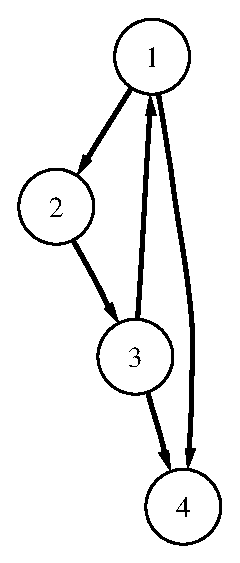
\includegraphics[bb=0 0 132
299]{graph} \end{center} \label{fig:graph} \end{figure}   

 

\subsection{\textcolor{Chapter }{RandomDiGraph}}
\logpage{[ "A", 1, 1 ]}\nobreak
\hyperdef{L}{X86CF9F66788B2A24}{}
{\noindent\textcolor{FuncColor}{$\triangleright$\ \ \texttt{RandomDiGraph({\mdseries\slshape n})\index{RandomDiGraph@\texttt{RandomDiGraph}}
\label{RandomDiGraph}
}\hfill{\scriptsize (function)}}\\


 Produces a pseudo random digraph with $n$ vertices 
\begin{Verbatim}[commandchars=!@|,fontsize=\small,frame=single,label=Example]
  !gapprompt@gap>| !gapinput@RandomDiGraph(4);|
  [ [  ], [ 1, 2, 4 ], [  ], [  ] ]
\end{Verbatim}
 }

 

\subsection{\textcolor{Chapter }{VertexInDegree}}
\logpage{[ "A", 1, 2 ]}\nobreak
\hyperdef{L}{X868EE741872B932D}{}
{\noindent\textcolor{FuncColor}{$\triangleright$\ \ \texttt{VertexInDegree({\mdseries\slshape DG, v})\index{VertexInDegree@\texttt{VertexInDegree}}
\label{VertexInDegree}
}\hfill{\scriptsize (function)}}\\


 Computes the in degree of the vertex \mbox{\texttt{\mdseries\slshape v}} of the directed graph \mbox{\texttt{\mdseries\slshape DG}} 
\begin{Verbatim}[commandchars=!@|,fontsize=\small,frame=single,label=Example]
  !gapprompt@gap>| !gapinput@G:=RandomDiGraph(4);|
  [ [ 1 ], [ 1, 2, 4 ], [  ], [ 1, 2, 3 ] ]
  !gapprompt@gap>| !gapinput@VertexInDegree(G,2);|
  2
\end{Verbatim}
 }

 

\subsection{\textcolor{Chapter }{VertexOutDegree}}
\logpage{[ "A", 1, 3 ]}\nobreak
\hyperdef{L}{X84DF2E8E7A7B32C6}{}
{\noindent\textcolor{FuncColor}{$\triangleright$\ \ \texttt{VertexOutDegree({\mdseries\slshape DG, v})\index{VertexOutDegree@\texttt{VertexOutDegree}}
\label{VertexOutDegree}
}\hfill{\scriptsize (function)}}\\


 Computes the out degree of the vertex \mbox{\texttt{\mdseries\slshape v}} of the directed graph \mbox{\texttt{\mdseries\slshape DG}} 
\begin{Verbatim}[commandchars=!@|,fontsize=\small,frame=single,label=Example]
  !gapprompt@gap>| !gapinput@G:=RandomDiGraph(4);|
  [ [ 1 ], [ 1, 2, 4 ], [  ], [ 1, 2, 3 ] ]
  !gapprompt@gap>| !gapinput@VertexOutDegree(G,2);|
  3
\end{Verbatim}
 }

 

\subsection{\textcolor{Chapter }{AutoVertexDegree}}
\logpage{[ "A", 1, 4 ]}\nobreak
\hyperdef{L}{X7FA6FAAE7AA8715D}{}
{\noindent\textcolor{FuncColor}{$\triangleright$\ \ \texttt{AutoVertexDegree({\mdseries\slshape DG, v})\index{AutoVertexDegree@\texttt{AutoVertexDegree}}
\label{AutoVertexDegree}
}\hfill{\scriptsize (function)}}\\


 Computes the degree of the vertex \mbox{\texttt{\mdseries\slshape v}} of the directed graph \mbox{\texttt{\mdseries\slshape DG}} 
\begin{Verbatim}[commandchars=!@|,fontsize=\small,frame=single,label=Example]
  !gapprompt@gap>| !gapinput@G:=RandomDiGraph(4);|
  [ [ 1 ], [ 1, 2, 4 ], [  ], [ 1, 2, 3 ] ]
  !gapprompt@gap>| !gapinput@AutoVertexDegree(G,2);|
  5
\end{Verbatim}
 }

 

\subsection{\textcolor{Chapter }{ReversedGraph}}
\logpage{[ "A", 1, 5 ]}\nobreak
\hyperdef{L}{X7BA5F1DF7DA89DC5}{}
{\noindent\textcolor{FuncColor}{$\triangleright$\ \ \texttt{ReversedGraph({\mdseries\slshape G})\index{ReversedGraph@\texttt{ReversedGraph}}
\label{ReversedGraph}
}\hfill{\scriptsize (function)}}\\


 Computes the reversed graph of the directed graph G. It is the graph obtained
from G by reversing the edges. 
\begin{Verbatim}[commandchars=!@|,fontsize=\small,frame=single,label=Example]
  !gapprompt@gap>| !gapinput@G:=RandomDiGraph(4);|
  [ [  ], [ 4 ], [ 2 ], [ 1, 4 ] ]
  !gapprompt@gap>| !gapinput@ReversedGraph(G);|
  [ [ 4 ], [ 3 ], [  ], [ 2, 4 ] ]
\end{Verbatim}
 }

 We say that a digraph is connected when for every pair of vertices there is a
path consisting of directed or reversed edges from one vertex to the other. 

\subsection{\textcolor{Chapter }{AutoConnectedComponents}}
\logpage{[ "A", 1, 6 ]}\nobreak
\hyperdef{L}{X7F23780E7A12A79E}{}
{\noindent\textcolor{FuncColor}{$\triangleright$\ \ \texttt{AutoConnectedComponents({\mdseries\slshape G})\index{AutoConnectedComponents@\texttt{AutoConnectedComponents}}
\label{AutoConnectedComponents}
}\hfill{\scriptsize (function)}}\\


 Computes a list of the connected components of the digraph 
\begin{Verbatim}[commandchars=!@|,fontsize=\small,frame=single,label=Example]
  !gapprompt@gap>| !gapinput@G:=RandomDiGraph(6);|
  [ [  ], [ 1, 4, 5, 6 ], [  ], [ 1, 3, 5, 6 ], [ 2, 3 ], [ 2, 4, 6 ] ]
  !gapprompt@gap>| !gapinput@AutoConnectedComponents(G);|
  [ [ 1, 2, 3, 4, 5, 6 ] ]
\end{Verbatim}
 }

 Two vertices of a digraph belong to a strongly connected component if there is
a directed path from each one to the other.

 

\subsection{\textcolor{Chapter }{GraphStronglyConnectedComponents}}
\logpage{[ "A", 1, 7 ]}\nobreak
\hyperdef{L}{X7D5288C982F92481}{}
{\noindent\textcolor{FuncColor}{$\triangleright$\ \ \texttt{GraphStronglyConnectedComponents({\mdseries\slshape G})\index{GraphStronglyConnectedComponents@\texttt{GraphStronglyConnectedComponents}}
\label{GraphStronglyConnectedComponents}
}\hfill{\scriptsize (function)}}\\


 Produces the strongly connected components of the digraph \mbox{\texttt{\mdseries\slshape G}}. 
\begin{Verbatim}[commandchars=!@|,fontsize=\small,frame=single,label=Example]
  !gapprompt@gap>| !gapinput@G:=RandomDiGraph(6);|
  [ [  ], [ 4 ], [  ], [ 4, 6 ], [  ], [ 1, 4, 5, 6 ] ]
  !gapprompt@gap>| !gapinput@GraphStronglyConnectedComponents(G);|
  [ [ 1 ], [ 2 ], [ 3 ], [ 4, 6 ], [ 5 ] ]
\end{Verbatim}
 }

 

\subsection{\textcolor{Chapter }{UnderlyingMultiGraphOfAutomaton}}
\logpage{[ "A", 1, 8 ]}\nobreak
\hyperdef{L}{X859B7C517AFBD198}{}
{\noindent\textcolor{FuncColor}{$\triangleright$\ \ \texttt{UnderlyingMultiGraphOfAutomaton({\mdseries\slshape A})\index{UnderlyingMultiGraphOfAutomaton@\texttt{UnderlyingMultiGraphOfAutomaton}}
\label{UnderlyingMultiGraphOfAutomaton}
}\hfill{\scriptsize (function)}}\\


 \mbox{\texttt{\mdseries\slshape A}} is an automaton. The output is the underlying directed multi-graph. 
\begin{Verbatim}[commandchars=!@B,fontsize=\small,frame=single,label=Example]
  !gapprompt@gap>B !gapinput@a:=RandomAutomaton("det",3,2);;Display(a);B
     |  1  2  3
  --------------
   a |  1  3
   b |     2  3
  Initial state:    [ 1 ]
  Accepting states: [ 1, 2 ]
  !gapprompt@gap>B !gapinput@UnderlyingMultiGraphOfAutomaton(a);B
  [ [ 1 ], [ 3, 2 ], [ 3 ] ]
\end{Verbatim}
 }

 

\subsection{\textcolor{Chapter }{UnderlyingGraphOfAutomaton}}
\logpage{[ "A", 1, 9 ]}\nobreak
\hyperdef{L}{X78CF8E507E100C62}{}
{\noindent\textcolor{FuncColor}{$\triangleright$\ \ \texttt{UnderlyingGraphOfAutomaton({\mdseries\slshape A})\index{UnderlyingGraphOfAutomaton@\texttt{UnderlyingGraphOfAutomaton}}
\label{UnderlyingGraphOfAutomaton}
}\hfill{\scriptsize (function)}}\\


 \mbox{\texttt{\mdseries\slshape A}} is an automaton. The output is the underlying directed graph. 
\begin{Verbatim}[commandchars=!@B,fontsize=\small,frame=single,label=Example]
  !gapprompt@gap>B !gapinput@a:=RandomAutomaton("det",3,2);;Display(a);B
     |  1  2  3
  --------------
   a |     1  2
   b |  1  2
  Initial state:   [ 2 ]
  Accepting state: [ 2 ]
  !gapprompt@gap>B !gapinput@UnderlyingGraphOfAutomaton(a);B
  [ [ 1 ], [ 1, 2 ], [ 2 ] ]
\end{Verbatim}
 }

 

\subsection{\textcolor{Chapter }{DiGraphToRelation}}
\logpage{[ "A", 1, 10 ]}\nobreak
\hyperdef{L}{X78869D478792B3AD}{}
{\noindent\textcolor{FuncColor}{$\triangleright$\ \ \texttt{DiGraphToRelation({\mdseries\slshape D})\index{DiGraphToRelation@\texttt{DiGraphToRelation}}
\label{DiGraphToRelation}
}\hfill{\scriptsize (function)}}\\


 Returns the relation corresponding to the digraph. Note that a directed graph
may be seen in a natural way as a binary relation on the set of vertices. 
\begin{Verbatim}[commandchars=!@|,fontsize=\small,frame=single,label=Example]
  !gapprompt@gap>| !gapinput@G:=RandomDiGraph(4);|
  [ [  ], [  ], [ 4 ], [ 4 ] ]
  !gapprompt@gap>| !gapinput@DiGraphToRelation(G);|
  [ [ 3, 4 ], [ 4, 4 ] ]
\end{Verbatim}
 }

 

\subsection{\textcolor{Chapter }{MSccAutomaton}}
\logpage{[ "A", 1, 11 ]}\nobreak
\hyperdef{L}{X7D63604A8413AAAF}{}
{\noindent\textcolor{FuncColor}{$\triangleright$\ \ \texttt{MSccAutomaton({\mdseries\slshape A})\index{MSccAutomaton@\texttt{MSccAutomaton}}
\label{MSccAutomaton}
}\hfill{\scriptsize (function)}}\\


 Produces an automaton where, in each strongly connected component, edges
labeled by inverses are added. (M stands for modified.) 

 This construction is useful in Finite Semigroup Theory. 
\begin{Verbatim}[commandchars=!@C,fontsize=\small,frame=single,label=Example]
  !gapprompt@gap>C !gapinput@a:=RandomAutomaton("det",3,2);;Display(a);C
     |  1  2  3
  --------------
   a |  1  3
   b |  2  3
  Initial state:    [ 1 ]
  Accepting states: [ 1, 2, 3 ]
  !gapprompt@gap>C !gapinput@MSccAutomaton(a);C
  < deterministic automaton on 4 letters with 3 states >
  !gapprompt@gap>C !gapinput@Display(last);C
     |  1  2  3
  --------------
   a |  1  3
   b |  2  3
   A |  1
   B |
  Initial state:    [ 1 ]
  Accepting states: [ 1, 2, 3 ]
\end{Verbatim}
 }

 

\subsection{\textcolor{Chapter }{AutoIsAcyclicGraph}}
\logpage{[ "A", 1, 12 ]}\nobreak
\hyperdef{L}{X7971EE367B6B7F36}{}
{\noindent\textcolor{FuncColor}{$\triangleright$\ \ \texttt{AutoIsAcyclicGraph({\mdseries\slshape G})\index{AutoIsAcyclicGraph@\texttt{AutoIsAcyclicGraph}}
\label{AutoIsAcyclicGraph}
}\hfill{\scriptsize (function)}}\\


 The argument is a graph's list of adjacencies and this function returns true
if the argument is an acyclic graph and false otherwise. 
\begin{Verbatim}[commandchars=!@|,fontsize=\small,frame=single,label=Example]
  !gapprompt@gap>| !gapinput@RandomDiGraph(3);|
  [ [  ], [ 3 ], [ 2 ] ]
  !gapprompt@gap>| !gapinput@AutoIsAcyclicGraph(last);|
  false
\end{Verbatim}
 }

 }

 }


\chapter{\textcolor{Chapter }{ Drawing automata }}\logpage{[ "B", 0, 0 ]}
\hyperdef{L}{X82D249F0793E6561}{}
{
  The drawing of graphs described here uses \texttt{graphviz} \cite{KoutsofiosNorth:2002}, a software for drawing graphs developed at AT  \&   T Labs, that can be obtained at \href{http://www.graphviz.org/} {\texttt{http://www.graphviz.org/}}. 
\section{\textcolor{Chapter }{ Installing some external programs }}\logpage{[ "B", 1, 0 ]}
\hyperdef{L}{X7988DBAB78EA0C06}{}
{
  In order to create the drawings you should install \href{http://www.graphviz.org/} {graphviz} and to view them you should install one of \href{http://www.gnome.org/projects/evince/} {evince}, \href{http://directory.fsf.org/GNU/ggv.html} {ggv}, \href{http://pages.cs.wisc.edu/~ghost/gsview/} {gsview} or \href{http://www.gnu.org/software/gv/} {gv}. }

 
\section{\textcolor{Chapter }{ Functions to draw automata }}\logpage{[ "B", 2, 0 ]}
\hyperdef{L}{X84C97CA079719B11}{}
{
  

\subsection{\textcolor{Chapter }{DrawAutomaton}}
\logpage{[ "B", 2, 1 ]}\nobreak
\hyperdef{L}{X7BC2FDA77FD0237B}{}
{\noindent\textcolor{FuncColor}{$\triangleright$\ \ \texttt{DrawAutomaton({\mdseries\slshape A[, state{\textunderscore}names, L, file]})\index{DrawAutomaton@\texttt{DrawAutomaton}}
\label{DrawAutomaton}
}\hfill{\scriptsize (function)}}\\


 This function draws automaton \mbox{\texttt{\mdseries\slshape A}}. The arguments \mbox{\texttt{\mdseries\slshape state{\textunderscore}names}}, \mbox{\texttt{\mdseries\slshape L}} and \mbox{\texttt{\mdseries\slshape file}} are optional. 

 An automaton with \texttt{n} states will be drawn with numbers \texttt{1} to \texttt{n} written inside the corresponding graph node. The argument \mbox{\texttt{\mdseries\slshape state{\textunderscore}names}} is a list of \texttt{n} strings which will be the new text written inside the corresponding graph
node. 

 The argument \mbox{\texttt{\mdseries\slshape L}} is a list of lists of integers, each of which specifies a set of states to be
drawn in a different color. 

 The argument \mbox{\texttt{\mdseries\slshape file}} is a string that specifies the name of the file containing the drawing. If it
is not give, it defaults to \texttt{"automaton"}. 
\begin{Verbatim}[commandchars=!@|,fontsize=\small,frame=single,label=Example]
  !gapprompt@gap>| !gapinput@x:=Automaton("det",3,2,[ [ 2, 3, 0 ], [ 0, 1, 2 ] ],[ 1 ],[ 1, 2, 3 ]);;|
  !gapprompt@gap>| !gapinput@DrawAutomaton(x,"file_name");|
  Displaying file: /tmp/tmp.Rj0v1s/file_name.dot.ps
  
  !gapprompt@gap>| !gapinput@DrawAutomaton(x,["st 1", "2", "C"],"file_name");|
  Displaying file: /tmp/tmp.BCH3FO/file_name.dot.ps
  
  !gapprompt@gap>| !gapinput@DrawAutomaton(x,["st 1", "2", "C"],[[2],[1,3]]);|
  Displaying file: /tmp/tmp.LPnJMq/automaton.dot.ps
\end{Verbatim}
 The output of the three previous \texttt{DrawAutomaton} commands would be the following diagrams displayed in a \emph{ghostview} window, respectively. 

  \begin{figure}[htbp] \begin{center} \leavevmode 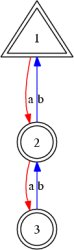
\includegraphics[bb=0 0 74
250]{aut2.jpg} \end{center} \label{fig:aut2} \end{figure}   

  \begin{figure}[htbp] \begin{center} \leavevmode 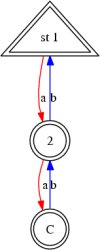
\includegraphics[bb=0 0 100
250]{aut2_1.jpg} \end{center} \label{fig:aut2_1} \end{figure}   

  \begin{figure}[htbp] \begin{center} \leavevmode 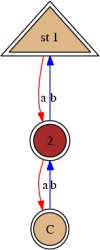
\includegraphics[bb=0 0 100
250]{aut2_2.jpg} \end{center} \label{fig:aut2_2} \end{figure}   

 }

 

\subsection{\textcolor{Chapter }{DrawAutomata}}
\logpage{[ "B", 2, 2 ]}\nobreak
\hyperdef{L}{X7AEE146D8391CA3D}{}
{\noindent\textcolor{FuncColor}{$\triangleright$\ \ \texttt{DrawAutomata({\mdseries\slshape A, B[, file]})\index{DrawAutomata@\texttt{DrawAutomata}}
\label{DrawAutomata}
}\hfill{\scriptsize (function)}}\\


 This function tests if automaton \texttt{ A } is a subautomaton of \texttt{ B } in which case draws \texttt{ B } highlighting the edges not in \texttt{ A } by drawing them in a dotted style, while the others are drawn in a plain
style. }

 

\subsection{\textcolor{Chapter }{DrawGraph}}
\logpage{[ "B", 2, 3 ]}\nobreak
\hyperdef{L}{X7D17B77F829F9CCB}{}
{\noindent\textcolor{FuncColor}{$\triangleright$\ \ \texttt{DrawGraph({\mdseries\slshape G[, file]})\index{DrawGraph@\texttt{DrawGraph}}
\label{DrawGraph}
}\hfill{\scriptsize (function)}}\\


 Draws a graph specified as an adjacency list \texttt{G}. }

 

\subsection{\textcolor{Chapter }{DrawSCCAutomaton}}
\logpage{[ "B", 2, 4 ]}\nobreak
\hyperdef{L}{X7E478FDD807853CA}{}
{\noindent\textcolor{FuncColor}{$\triangleright$\ \ \texttt{DrawSCCAutomaton({\mdseries\slshape A[, state{\textunderscore}names, L, file]})\index{DrawSCCAutomaton@\texttt{DrawSCCAutomaton}}
\label{DrawSCCAutomaton}
}\hfill{\scriptsize (function)}}\\


 Draws automaton \texttt{ A } and highlights it's strongly connected components by drawing the other edges
in a dotted style. 

 The optional arguments \mbox{\texttt{\mdseries\slshape state{\textunderscore}names}}, \mbox{\texttt{\mdseries\slshape L}} and \mbox{\texttt{\mdseries\slshape file}} are as described in \texttt{DrawAutomaton} (\ref{DrawAutomaton}). }

 }

 
\section{\textcolor{Chapter }{Drawings output formats}}\logpage{[ "B", 3, 0 ]}
\hyperdef{L}{X7F5419527FFCD1DF}{}
{
  Since drawings are mostly used in the \textsf{SgpViz} package, please refer to that package's \href{http://www.gap-system.org/Manuals/pkg/sgpviz/doc/manual.html} {manual} section of the same name. }

 
\section{\textcolor{Chapter }{Drawings extra graph attributes}}\logpage{[ "B", 4, 0 ]}
\hyperdef{L}{X795DD98D86A1A441}{}
{
  Since drawings are mostly used in the \textsf{SgpViz} package, please refer to that package's \href{http://www.gap-system.org/Manuals/pkg/sgpviz/doc/manual.html} {manual} section of the same name. }

 }


\chapter{\textcolor{Chapter }{Inverse automata and subgroups of the free group}}\logpage{[ "C", 0, 0 ]}
\hyperdef{L}{X7DBBB0537ADC9899}{}
{
 Inverse automata with a single initial/accepting state are in a one to one
correspondence with finitely generated subgroups of the free group over the
alphabet of the automaton. See \cite{MSW:2001}, \cite{KM:2002} for details, as well as for concepts such as \emph{flower automaton} and \emph{Stallings foldings}. 
\section{\textcolor{Chapter }{From subgroups to inverse automata}}\logpage{[ "C", 1, 0 ]}
\hyperdef{L}{X7DDDA5127A3D170C}{}
{
 A finitely generated subgroup of a finitely generated free group is given
through a list whose first element is the number of generators of the free
group and the remaining elements are the generators of the subgroup. The set
of generators of the free group of rank $n$ consists on the $n$ first letters of the set $\{a,b,c,d,e,f,g\}$. In particular, free groups of rank greater than $8$ must not be considered. A formal inverse of a generator is represented by the
corresponding capital letter. 

 A generator of the subgroup may be given through a string of letters or
through a list of positive integers as should be clear from the example that
follows. 

 For example, \texttt{[2,"abA","bbabAB"]} stands for the subgroup of the free group of rank 2 on the generators $aba^{-1}$ and $bbaba^{-1}b^{-1}$. The same subgroup may be given as \texttt{[2,[1,2,3],[2,2,1,2,3,4]]}. The number $ n+j$ represents the formal inverse of the generator represented by $j$. One can go from one representation to another, using the following
functions. 

\subsection{\textcolor{Chapter }{GeneratorsToListRepresentation}}
\logpage{[ "C", 1, 1 ]}\nobreak
\hyperdef{L}{X85358D097C314EB5}{}
{\noindent\textcolor{FuncColor}{$\triangleright$\ \ \texttt{GeneratorsToListRepresentation({\mdseries\slshape L})\index{GeneratorsToListRepresentation@\texttt{GeneratorsToListRepresentation}}
\label{GeneratorsToListRepresentation}
}\hfill{\scriptsize (function)}}\\


 
\begin{Verbatim}[commandchars=!@|,fontsize=\small,frame=single,label=Example]
  !gapprompt@gap>| !gapinput@L:=[2,"abA","bbabAB"];;|
  !gapprompt@gap>| !gapinput@GeneratorsToListRepresentation(L);|
  [ 2, [ 1, 2, 3 ], [ 2, 2, 1, 2, 3, 4 ] ]
\end{Verbatim}
 }

 

\subsection{\textcolor{Chapter }{ListToGeneratorsRepresentation}}
\logpage{[ "C", 1, 2 ]}\nobreak
\hyperdef{L}{X80F3E10784590374}{}
{\noindent\textcolor{FuncColor}{$\triangleright$\ \ \texttt{ListToGeneratorsRepresentation({\mdseries\slshape K})\index{ListToGeneratorsRepresentation@\texttt{ListToGeneratorsRepresentation}}
\label{ListToGeneratorsRepresentation}
}\hfill{\scriptsize (function)}}\\


 
\begin{Verbatim}[commandchars=!@|,fontsize=\small,frame=single,label=Example]
  !gapprompt@gap>| !gapinput@K:=[2,[1,2,3],[2,2,1,2,3,4]];;|
  !gapprompt@gap>| !gapinput@ListToGeneratorsRepresentation(K);|
  [ 2, "abA", "bbabAB" ]
\end{Verbatim}
 }

 

\subsection{\textcolor{Chapter }{FlowerAutomaton}}
\logpage{[ "C", 1, 3 ]}\nobreak
\hyperdef{L}{X7EAFF7E879D115C5}{}
{\noindent\textcolor{FuncColor}{$\triangleright$\ \ \texttt{FlowerAutomaton({\mdseries\slshape L})\index{FlowerAutomaton@\texttt{FlowerAutomaton}}
\label{FlowerAutomaton}
}\hfill{\scriptsize (function)}}\\


 The argument \texttt{L} is a subgroup of the free group given through any of the representations
described above. Returns the flower automaton. 
\begin{Verbatim}[commandchars=!@C,fontsize=\small,frame=single,label=Example]
  !gapprompt@gap>C !gapinput@W:=[2,"bbbAB","abAbA"];;C
  !gapprompt@gap>C !gapinput@A:=FlowerAutomaton(W);C
  < non deterministic automaton on 2 letters with 9 states >
  !gapprompt@gap>C !gapinput@Display(A);C
     |  1          2       3       4    5       6       7    8       9
  ---------------------------------------------------------------------
   a | [ 6, 9 ]                        [ 4 ]                [ 7 ]
   b | [ 2, 5 ]   [ 3 ]   [ 4 ]                [ 7 ]        [ 9 ]
  Initial state:   [ 1 ]
  Accepting state: [ 1 ]
\end{Verbatim}
 }

 

\subsection{\textcolor{Chapter }{FoldFlowerAutomaton}}
\logpage{[ "C", 1, 4 ]}\nobreak
\hyperdef{L}{X7F729A4E8784D92E}{}
{\noindent\textcolor{FuncColor}{$\triangleright$\ \ \texttt{FoldFlowerAutomaton({\mdseries\slshape A})\index{FoldFlowerAutomaton@\texttt{FoldFlowerAutomaton}}
\label{FoldFlowerAutomaton}
}\hfill{\scriptsize (function)}}\\


 Makes identifications on the flower automaton \texttt{A}. In the literature, these identifications are called Stallings foldings. 

 (This function may have \texttt{true} as a second argument. WARNING: the second argument should only be used when
facilities to draw automata are available. In that case, one may visualize the
identifications that are taking place.) 
\begin{Verbatim}[commandchars=!@C,fontsize=\small,frame=single,label=Example]
  !gapprompt@gap>C !gapinput@B := FoldFlowerAutomaton(A);C
  < deterministic automaton on 2 letters with 7 states >
  !gapprompt@gap>C !gapinput@Display(B);C
     |  1  2  3  4  5  6  7
  --------------------------
   a |  5  4              6
   b |  2  3  4     6     5
  Initial state:   [ 1 ]
  Accepting state: [ 1 ]
\end{Verbatim}
 }

 

\subsection{\textcolor{Chapter }{SubgroupGenToInvAut}}
\logpage{[ "C", 1, 5 ]}\nobreak
\hyperdef{L}{X826D581D794F1BFB}{}
{\noindent\textcolor{FuncColor}{$\triangleright$\ \ \texttt{SubgroupGenToInvAut({\mdseries\slshape L})\index{SubgroupGenToInvAut@\texttt{SubgroupGenToInvAut}}
\label{SubgroupGenToInvAut}
}\hfill{\scriptsize (function)}}\\


 Returns the inverse automaton corresponding to the subgroup given by \mbox{\texttt{\mdseries\slshape L}}. 
\begin{Verbatim}[commandchars=!@C,fontsize=\small,frame=single,label=Example]
  !gapprompt@gap>C !gapinput@L:=[2,"bbbAB","AbAbA"];;C
  !gapprompt@gap>C !gapinput@SubgroupGenToInvAut(L);C
  < deterministic automaton on 2 letters with 8 states >
  !gapprompt@gap>C !gapinput@Display(last);C
     |  1  2  3  4  5  6  7  8
  -----------------------------
   a |  8  4        1     6
   b |  2  3  4     6     8
  Initial state:   [ 1 ]
  Accepting state: [ 1 ]
  
\end{Verbatim}
 }

 }

 
\section{\textcolor{Chapter }{From inverse automata to subgroups}}\logpage{[ "C", 2, 0 ]}
\hyperdef{L}{X85F2060A86DBE62B}{}
{
 Given an inverse automaton with a single initial/accepting state, one can find
a set of generators for the subgroup represented by the automaton. Moreover,
using a geodesic tree, one can find a Nielsen reduced set of generators \cite{KM:2002}. 

\subsection{\textcolor{Chapter }{GeodesicTreeOfInverseAutomaton}}
\logpage{[ "C", 2, 1 ]}\nobreak
\hyperdef{L}{X81DA149779A167BD}{}
{\noindent\textcolor{FuncColor}{$\triangleright$\ \ \texttt{GeodesicTreeOfInverseAutomaton({\mdseries\slshape A})\index{GeodesicTreeOfInverseAutomaton@\texttt{GeodesicTreeOfInverseAutomaton}}
\label{GeodesicTreeOfInverseAutomaton}
}\hfill{\scriptsize (function)}}\\


 Returns a subautomaton of \mbox{\texttt{\mdseries\slshape A}}whose underlying graph is a geodesic tree of the underlying graph of the
inverse automaton \texttt{A}. 
\begin{Verbatim}[commandchars=!@B,fontsize=\small,frame=single,label=Example]
  !gapprompt@gap>B !gapinput@A:=Automaton("det",4,2,[ [ 3, 4, 0, 0 ], [ 2, 3, 4, 0 ] ],[ 1 ],[ 1 ]);;B
  !gapprompt@gap>B !gapinput@G := GeodesicTreeOfInverseAutomaton(A);B
  < deterministic automaton on 2 letters with 4 states >
  !gapprompt@gap>B !gapinput@Display(G);B
     |  1  2  3  4
  -----------------
   a |  3
   b |  2     4
  Initial state:   [ 1 ]
  Accepting state: [ 1 ]
\end{Verbatim}
 }

 

\subsection{\textcolor{Chapter }{InverseAutomatonToGenerators}}
\logpage{[ "C", 2, 2 ]}\nobreak
\hyperdef{L}{X7F117C43814F2CDE}{}
{\noindent\textcolor{FuncColor}{$\triangleright$\ \ \texttt{InverseAutomatonToGenerators({\mdseries\slshape A})\index{InverseAutomatonToGenerators@\texttt{InverseAutomatonToGenerators}}
\label{InverseAutomatonToGenerators}
}\hfill{\scriptsize (function)}}\\


 Returns a set of generators (given trough the representation above) of the
subgroup of the free group corresponding to the automaton \texttt{A} given. 
\begin{Verbatim}[commandchars=!@|,fontsize=\small,frame=single,label=Example]
  !gapprompt@gap>| !gapinput@NW := InverseAutomatonToGenerators(A);|
  [ 2, "baBA", "bbA" ]
\end{Verbatim}
 }

 }

 }

\def\bibname{References\logpage{[ "Bib", 0, 0 ]}
\hyperdef{L}{X7A6F98FD85F02BFE}{}
}

\bibliographystyle{alpha}
\bibliography{AutMan}

\addcontentsline{toc}{chapter}{References}

\def\indexname{Index\logpage{[ "Ind", 0, 0 ]}
\hyperdef{L}{X83A0356F839C696F}{}
}

\cleardoublepage
\phantomsection
\addcontentsline{toc}{chapter}{Index}


\printindex

\newpage
\immediate\write\pagenrlog{["End"], \arabic{page}];}
\immediate\closeout\pagenrlog
\end{document}
